\documentclass[english,a4paper,11pt,twoside,openany]{memoir} 	% Openright aabner kapitler paa hoejresider (openany begge)

%%%% PACKAGES %%%%

% ¤¤ Oversaettelse og tegnsaetning ¤¤ %
\usepackage[utf8x]{inputenc}					% Input-indkodning af tegnsaet (UTF8)
\usepackage[english]{babel}					% Dokumentets sprog
\usepackage[T1]{fontenc}					% Output-indkodning af tegnsaet (T1)
\usepackage{ragged2e,anyfontsize}			% Justering af elementer
%\usepackage{fixltx2e}						% Retter forskellige fejl i LaTeX-kernen
\usepackage{lastpage}
\usepackage{placeins}	
% font
\usepackage{charter}	
																
% ¤¤ Figurer og tabeller (floats) ¤¤ %
\usepackage{titlepic}
\usepackage{graphicx} 						% Haandtering af eksterne billeder (JPG, PNG, PDF)

\usepackage{subcaption}
\usepackage{multirow,booktabs}              % Fletning af raekker og kolonner (\multicolumn og \multirow)
\usepackage{colortbl} 						% Farver i tabeller (fx \columncolor, \rowcolor og \cellcolor)
\usepackage[dvipsnames]{xcolor}				% Definer farver med \definecolor. Se mere: http://en.wikibooks.org/wiki/LaTeX/Colors
\usepackage{flafter}						% Soerger for at floats ikke optraeder i teksten foer deres reference
\let\newfloat\relax 						% Justering mellem float-pakken og memoir
%flyttet%\usepackage{float}							% Muliggoer eksakt placering af floats, f.eks. \begin{figure}[H]
\usepackage{rotating}
\usepackage{pdflscape}
\usepackage{array,booktabs,arydshln}		% 'arydshlyn' muliggør stiblede linier i tabeller med komandoen \hdashline
\usepackage{threeparttable}
\usepackage{lscape}
\usepackage{placeins}
%\usepackage{caption}
\usepackage{color}
%\usepackage{eso-pic}						% Tilfoej billedekommandoer paa hver side
\usepackage{makecell}			% Muligoer flere linjer i en celle i tabel
%\usepackage{wrapfig}						% Indsaettelse af figurer omsvoebt af tekst. \begin{wrapfigure}{Placering}{Stoerrelse}
%\usepackage{multicol}         	        	% Muliggoer tekst i spalter
%\usepackage{rotating}						% Rotation af tekst med \begin{sideways}...\end{sideways}

% ¤¤ Matematik mm. ¤¤
\usepackage{amsmath,amssymb,stmaryrd} 		% Avancerede matematik-udvidelser
\usepackage{mathtools}						% Andre matematik- og tegnudvidelser
\usepackage{textcomp}                 		% Symbol-udvidelser (f.eks. promille-tegn med \textperthousand )
\usepackage{siunitx}						% Flot og konsistent praesentation af tal og enheder med \si{enhed} og \SI{tal}{enhed}
\sisetup{output-decimal-marker = {,}}		% Opsaetning af \SI (DE for komma som decimalseparator) 
\usepackage[version=3]{mhchem} 				% Kemi-pakke til flot og let notation af formler, f.eks. \ce{Fe2O3}
%\usepackage{rsphrase}						% Kemi-pakke til RS-saetninger, f.eks. \rsphrase{R1}
\usepackage{amsmath}
\usepackage{cases}


% ¤¤ Referencer og kilder ¤¤ %
\usepackage[english]{varioref}				% Muliggoer bl.a. krydshenvisninger med sidetal (\vref)
\usepackage[square,numbers]{natbib}			% Udvidelse med naturvidenskabelige citationsmodeller		
%\usepackage{xr}							% Referencer til eksternt dokument med \externaldocument{<NAVN>}
%\usepackage{glossaries}					% Terminologi- eller symbolliste (se mere i Daleifs Latex-bog)
\usepackage{subfiles}
\usepackage{titletoc}

% ¤¤ Misc. ¤¤ %
\usepackage{listings}						% Placer kildekode i dokumentet med \begin{lstlisting}...\end{lstlisting}
\usepackage{lipsum}							% Dummy text \lipsum[..]
\usepackage[shortlabels]{enumitem}			% Muliggoer enkelt konfiguration af lister
\usepackage{pdfpages}						% Goer det muligt at inkludere pdf-dokumenter med kommandoen \includepdf[pages={x-y}]{fil.pdf}	
\pdfoptionpdfminorversion=6					% Muliggoer inkludering af pdf dokumenter, af version 1.6 og hoejere
\pretolerance=2500 							% Justering af afstand mellem ord (hoejt tal, mindre orddeling og mere luft mellem ord)
\usepackage{xspace}
% Kommentarer og rettelser med \fxnote. Med 'final' i stedet for 'draft' udloeser hver note en error i den faerdige rapport.
\usepackage[footnote,draft,english,draft,nomargin]{fixme}		
\usepackage{placeins}


%%%% CUSTOM SETTINGS %%%%

% ¤¤ Marginer ¤¤ %
\setlrmarginsandblock{3.3cm}{3.3cm}{*}		% \setlrmarginsandblock{Indbinding}{Kant}{Ratio}
\setulmarginsandblock{2.5cm}{3.0cm}{*}		% \setulmarginsandblock{Top}{Bund}{Ratio}
%\setlength{\headheight}{1.8cm}
\checkandfixthelayout 						% Oversaetter vaerdier til brug for andre pakker

%	¤¤ Afsnitsformatering ¤¤ %
\setlength{\parindent}{0mm}           		% Stoerrelse af indryk
\setlength{\parskip}{3mm}          			% Afstand mellem afsnit ved brug af double Enter
\linespread{1,0}							% Linie afstand

% ¤¤ Litteraturlisten ¤¤ %
%\bibpunct[,]{[}{]}{;}{a}{,}{,} 				% Definerer de 6 parametre ved Harvard henvisning (bl.a. parantestype og seperatortegn)
%\bibliographystyle{harvard}			% Udseende af litteraturlisten.
%\bibliographystyle{ksfh_nat}
%\bibliographystyle{abbrvnat}
\bibliographystyle{unsrt}
% ¤¤ Indholdsfortegnelse ¤¤ %
\setsecnumdepth{section}		 			% Dybden af nummerede overkrifter (part/chapter/section/subsection)
\maxsecnumdepth{section}					% Dokumentklassens graense for nummereringsdybde
\settocdepth{section} 					% Dybden af indholdsfortegnelsen

% ¤¤ Lister ¤¤ %
\setlist{
  topsep=0pt,								% Vertikal afstand mellem tekst og listen
  itemsep=-1ex,								% Vertikal afstand mellem items
} 


% ¤¤ Opsaetning af figur- og tabeltekst ¤¤ %
\captionnamefont{\small\bfseries\itshape}	% Opsaetning af tekstdelen ('Figur' eller 'Tabel')
\captiontitlefont{\small}					% Opsaetning af nummerering
\captiondelim{. }							% Seperator mellem nummerering og figurtekst
\captionsetup{font=footnotesize}
\hangcaption								% Venstrejusterer flere-liniers figurtekst under hinanden
%\captionwidth{\linewidth}					% Bredden af figurteksten
\setlength{\belowcaptionskip}{0pt}			% Afstand under figurteksten
		
% ¤¤ Opsaetning af listings ¤¤ %
\definecolor{commentGreen}{RGB}{34,139,24}
\definecolor{stringPurple}{RGB}{208,76,239}

\lstset{language=Matlab,					% Sprog
	basicstyle=\ttfamily\scriptsize,		% Opsaetning af teksten
	keywords={for,if,while,else,elseif,		% Noegleord at fremhaeve
			  end,break,return,case,
			  switch,function},
	keywordstyle=\color{blue},				% Opsaetning af noegleord
	commentstyle=\color{commentGreen},		% Opsaetning af kommentarer
	stringstyle=\color{stringPurple},		% Opsaetning af strenge
	showstringspaces=false,					% Mellemrum i strenge enten vist eller blanke
	numbers=left, numberstyle=\tiny,		% Linjenumre
	extendedchars=true, 					% Tillader specielle karakterer
	columns=flexible,						% Kolonnejustering
	breaklines, breakatwhitespace=true,		% Bryd lange linjer
}

% ¤¤ Navngivning ¤¤ %
\addto\captionsdanish{
	\renewcommand\appendixname{Bilag}
	\renewcommand\contentsname{Indholdsfortegnelse}	
	\renewcommand\appendixpagename{\appendixname~}
	\renewcommand\appendixtocname{\appendixname~}
	\renewcommand\cftchaptername{ }				% Skriver "Appendix" foran kapitlerne i indholdsfortegnelsen
	\renewcommand\cftappendixname{\appendixname~}			% Skriver "Bilag" foran appendiks i indholdsfortegnelsen
}

% ¤¤ Kapiteludssende ¤¤ %
%\definecolor{numbercolor}{gray}{0.7}		% Definerer en farve til brug til kapiteludseende
%\newif\ifchapternonum
%\makechapterstyle{hangnum}{					% Definerer kapiteludseende frem til ...
%  \renewcommand\beforechapskip{0pt}
%  \renewcommand\printchaptername{}
%  \renewcommand\printchapternum{}
%  \renewcommand\printchapternonum{\chapternonumtrue}
%  \renewcommand\chaptitlefont{\fontfamily{pbk}\fontseries{db}\fontshape{n}\fontsize{25}{35}%\selectfont\raggedleft}
%  \renewcommand\chapnumfont{\fontfamily{pbk}\fontseries{m}\fontshape{n}\fontsize{1in}{0in}\selectfont%\color{numbercolor}}
%  \renewcommand\printchaptertitle[1]{%
%    \noindent
%    \ifchapternonum
%    \begin{tabularx}{\textwidth}{X}
%    {\let\\\newline\chaptitlefont ##1\par} 
%    \end{tabularx}
%    \par\vskip-2.5mm\hrule
%    \else
%    \begin{tabularx}{\textwidth}{Xl}
%    {\parbox[b]{\linewidth}{\chaptitlefont ##1}} & \raisebox{-15pt}{\chapnumfont \thechapter}
%    \end{tabularx}
%    \par\vskip2mm\hrule
%    \fi
%  }
%}											% ... her

%\chapterstyle{hangnum}
\chapterstyle{southall}
\renewcommand\afterchapskip{0pt}
\renewcommand\beforechapskip{-25pt}						% Valg af kapiteludseende - Google 'memoir chapter styles' for alternativer

% ¤¤ Sidehoved ¤¤ %

\makepagestyle{Uni}							% Definerer sidehoved og sidefod udseende frem til ...
\makepsmarks{Uni}{%
	\createmark{chapter}{left}{shownumber}{}{. \ }
	\createmark{section}{right}{shownumber}{}{. \ }
	\createplainmark{toc}{both}{\contentsname}
	\createplainmark{lof}{both}{\listfigurename}
	\createplainmark{lot}{both}{\listtablename}
	\createplainmark{bib}{both}{\bibname}
	\createplainmark{index}{both}{\indexname}
	\createplainmark{glossary}{both}{\glossaryname}
}
\nouppercaseheads											% Ingen Caps oenskes

\makeevenhead{Uni}{\leftmark}{}{\rightmark}				% Definerer lige siders sidehoved (\makeevenhead{Navn}{Venstre}{Center}{Hoejre})
\makeoddhead{Uni}{}{}{}			% Definerer ulige siders sidehoved (\makeoddhead{Navn}{Venstre}{Center}{Hoejre})
\makeevenfoot{Uni}{Page{ }\thepage{ }of{ }\pageref*{LastPage}}{}{}							% Definerer lige siders sidefod (\makeevenfoot{Navn}{Venstre}{Center}{Hoejre})
\makeoddfoot{Uni}{}{}{Page{ }\thepage{ }of{ }\pageref*{LastPage}}								% Definerer ulige siders sidefod (\makeoddfoot{Navn}{Venstre}{Center}{Hoejre})
\makeheadrule{Uni}{\textwidth}{0pt}						% Tilfoejer en streg under sidehovedets indhold	
\makefootrule{Uni}{\textwidth}{0pt}{1mm}					% Tilfoejer en streg under sidefodens indhold

\copypagestyle{Unichap}{Uni}								% Sidehoved for kapitelsider defineres som standardsider, men med blank sidehoved
\makeoddhead{Unichap}{}{}{}
\makeevenhead{Unichap}{}{}{}
\makeheadrule{Unichap}{\textwidth}{0pt}
\aliaspagestyle{chapter}{Unichap}							% Den ny style vaelges til at gaelde for chapters
															% ... her
															
\pagestyle{Uni}												% Valg af sidehoved og sidefod (benyt "plain" for ingen sidehoved/fod)


%%%% CUSTOM COMMANDS %%%%

% ¤¤ Billede hack ¤¤ %										% Indsaet figurer nemt med \figur{Stoerrelse}{Fil}{Figurtekst}{Label}
\newcommand{\figur}[4]{
		\begin{figure}[H] \centering
			\includegraphics[width=#1\textwidth]{billeder/#2}
			\caption{#3}\label{#4}
		\end{figure} 
}

% ¤¤ Specielle tegn ¤¤ %
\newcommand{\decC}{^{\circ}\text{C}}
\newcommand{\dec}{^{\circ}\text{C}}
\newcommand{\m}{\cdot}


%%%% ORDDELING %%%%

\hyphenation{}

%%%%%BILAG - FORSØG%%%%

% ¤¤ Visuelle referencer ¤¤ %
\usepackage[colorlinks,hypertexnames=false]{hyperref}			% Danner klikbare referencer (hyperlinks) i dokumentet.
\hypersetup{colorlinks = true,				% Opsaetning af farvede hyperlinks (interne links, citeringer og URL)
	linkcolor = black,
	citecolor = black,
	urlcolor = black
,bookmarksopen=false}
\usepackage[
open,
openlevel=-1,
atend
]{bookmark}
\usepackage{float}	
\usepackage{soul}

\newcommand{\tc}{\textcelsius \xspace}
\newcommand{\EE}[1]{\ensuremath{\cdot 10^{#1}}}
\newcommand{\gange}{\ensuremath{\cdot}} %disse to er til at sikre SIunitx virker som vi vil ha
\renewcommand{\times}{\cdot}

\usepackage[official]{eurosym}
\usepackage{changepage}

\usepackage{import}
\usepackage{xifthen}
\usepackage{pdfpages}
\usepackage{transparent}
\usepackage{pdfpages}

\newcommand{\incfig}[1]{%
	\def\svgwidth{\columnwidth}
	\import{./Images/}{#1.pdf_tex}
}



\title{\Huge A novel modeling to generate alternatives approach: Determining the convex hull containing all near optimal solutions}
\author{ Tim T. Pedersen}
\date{ January 2020}
\titlepic{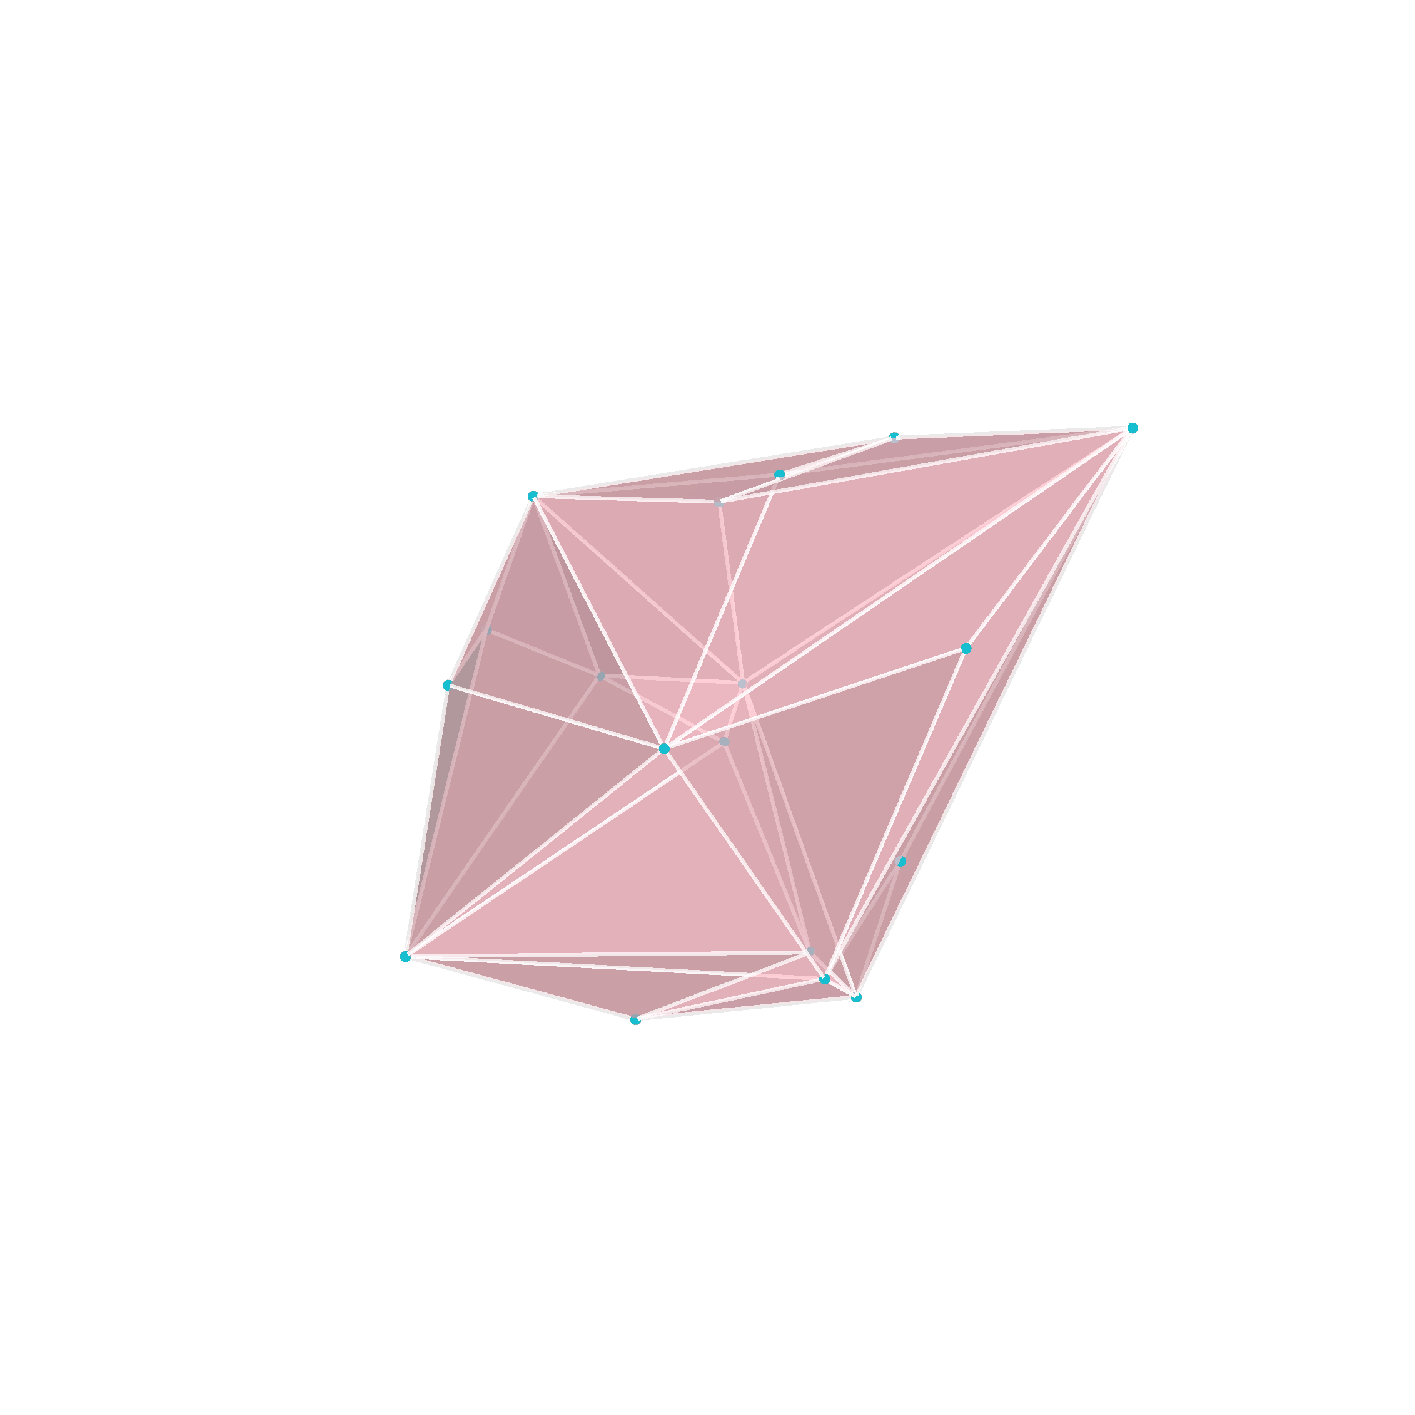
\includegraphics[width=.8\linewidth,trim={6cm 6cm 4cm 4cm},clip]{Images/title_pic.pdf}}



\begin{document}
	
\frontmatter
\pagenumbering{gobble}
\maketitle

\clearpage
\pagenumbering{roman}

\vspace{3.5cm}
{\Huge\textbf{Title page}} \\
\rule{1.0\textwidth}{0.1mm}\\ %Skillelinje

\textbf{Title:}\\
A novel modeling to generate alternatives approach: Determining the convex hull containing all near optimal solutions \\

\textbf{Project:}\\
Mester's Thesis, Department of Engineering , Aarhus University.

\textbf{Date finished:}\\ 3rd January 2020

\textbf{Author:}\\ 
Tim Tørnes Pedersen - 201403848 - au518895\\

\textbf{Project supervisors:}\\
Gorm B. Andresen, Associate professor,  Department of Engineering, Aarhus University\\ 
Marta Victoria, Assistant Professor, Department of Engineering, Aarhus University\\\\ \\


This project is lawfully written by the following author:

\begin{figure}[H]

\includegraphics[width=0.45\textwidth]{./Images/underskrift}
\end{figure}

%\rule{.5\textwidth}{0.1mm}\\ %Skillelinje
%\small{Cecilie Viborg Nielsen}\\ \\

%\rule{.5\textwidth}{0.1mm}\\ %Skillelinje
%\small{Tim Tørnes Pedersen}\\ \\ \\ \\ \\

\textit{The content of this project is freely available, but publication (with references) must only be done with an agreement with the authors.}

\newpage

\clearpage

\chapter{Abstract}

\begin{adjustwidth}{-10pt}{-20pt}


% Problem 
% - CO2 emissions must be reduced to prevent climate change 
% - Energy-economic modeling as tool to decrease CO2 emission 
% - How model optimizations is used today
% - Large uncertainty in model structure and input data = large uncertainty in results
% - HSJ MGA 
To limit the extent of irreversible climate change and accepting public opinion expressed in Greta Thunberg's speech at the UN Climate Action summit, drastic measures are needed to reduce the emission of greenhouse gases. The majority of CO2 emitted by humans are results of energy production to cover the ever-rising energy demand including transportation, heating, and electricity. To assist scientists and policymakers in their stride to reach ambitious goals in the reduction of CO2 emissions, analysis tools must be developed. An important tool, when it comes to planning of global and local energy networks are numeric techno-economic energy models. These models are capable of providing great insight into complex systems such as the European electricity grid and allows the user to make predictions about future needs and design strategies. 

Numeric energy-economic models do however suffer from great uncertainties arising from flaws in the mathematical formulation and construction of the energy-economic model referred to as structural uncertainty. An example of flaws in the mathematical formulation, could be unmodeled constraints such as public acceptance issues.
If these uncertainties are not addressed, the results become untrustworthy and ends up providing little to no insight.
Until recently, no methods for addressing structural uncertainty of the techno-economic models existed. This changed in 2010 when J. DeCarolis published a paper proposing a technique called "Modeling to generate alternatives (MGA)" doing just so. The root cause of structural uncertainty cannot be addressed as it can with parametric uncertainty, as the origin of structural uncertainty is hard to define. Instead one must investigate all solutions near the one found to be optimal, and estimate the likelihood of these near optimal solutions being the true optimal solution. 
%In the technique proposed by J. DeCarolis, a finite set of maximally different near-optimal solutions are found. The difference in the found solutions can then be used as a measure of structural uncertainty and provides a variety of alternatives to the optimal configuration of the energy system. 

% Objective 
% - Study the nature of the near optimal feasible space
% - Define MGA approach that will search evenly across the near optimal feasible space
The proposed technique by J. DeCarolis does however, suffer from a range of flaws, arising from lacking structure in the manner near-optimal solutions are found. To obtain a complete picture of all near optimal solutions, a structured method of finding these is needed. 
The objective of this thesis is to explore the characteristics of all near optimal solutions contained within the near-optimal feasible decision space, and to develop a new technique that in a structured manner can explore all solutions located within this space.  

% Methodology 

% Results
% - MGA shows as a feasible tool 
% - Multiplicity is wery important to consider 
Analysis of the common mathematical formulation of numeric techno-economic model reveal that the model consists of linear constraints and therefore, the near-optimal feasible decision space, containing all near optimal solutions to the model, must be convex. 
Knowing these properties, a technique has been developed capable of searching the entire near optimal feasible decision space. The technique iteratively converges towards the full solution, and provides statistical information about all near optimal solutions. 
Furthermore, a method reducing the complexity of the mathematical problem, by grouping of variables is proposed. Grouping the variables in the model to form a new set of variables, does however reduce the amount of information obtained by solving this simplified problem. The effects of grouping the model variables is explored, and the effect is found to be significant, but predictable. 

% Conclusion 
% - An MGA approach has been developed
The developed method is applied to a model of the European electricity grid. The usefulness of the technique is proven as it provides information about the distribution of technology capacities in all near optimal solutions to the used model of the European electricity gird. 



\end{adjustwidth}








\mainmatter
%\phantomsection
%\mainmatter
\startlist{toc}\thispagestyle{empty}
\printlist{toc}{}{\part{Main Report}\clearpage}
%\addtocontents{toc}{part}{Hovedrapport}
\setcounter{chapter}{0}
\renewcommand{\thechapter}{\arabic{chapter}}

\listoffixmes

\clearpage

\chapter{Introduction}

%\subsection{Problem definition}

% Large Scale Background
High global ambitions for decreased CO2 emission and the resulting increase in implementation of renewable energy sources, introduce higher demands to the energy grid than ever. The volatile nature of renewable energy sources, implemented to reach ambitious CO2 emission goals, drives the need for collaboration/coupling between countries, energy sectors, and energy sources, to handle peak loads and hours of energy scarcity. This complicates the already complex task of energy system synthesis even further, hereby requiring decision makers to have greater in depth knowledge, in a world where rapid decisions and superficial political decisions are becoming more widespread. Therefore, the need for analysis tools providing insights in the constraints and possibilities decision makers must deal with, has never been more present.  

% Narrow background
A frequently used tool to gain insight in the future energy grid compositions, is energy-economic models on either regional, national or international scale. These models can be used to study the behavior and composition of existing and future energy networks, together with the impact of new technologies or structural changes in the networks \cite{Gorm_impact_of_CO2_PYPSA} !!CITE OTHEER WORKS USING energy-economic models!!. 
However, these models do suffer from large uncertainties and the lack of validation possibilities, resulting in unreliable and therefore less informative results. 

Model uncertainty can be categorized as either parametric uncertainty, arising from uncertainty in input parameters and data, or as structural uncertainty introduced by an incomplete or faulty mathematical description of the problem at hand \cite{DeCarolis_MGA} . Structural uncertainty is however not caused by the modelers lack of mathematical talent, but is the result of dealing with a very complex problem, influenced by multiple actors such as policymakers and private company's in the energy sector. 

% Literature review/Current standpoint
Recently an approach for extracting more relevant and less uncertain data from energy-economic models has been proposes by \citeauthor{DeCarolis_MGA}, where a technique called Modeling to Generate Alternatives (MGA), from the field of management research/planning science \cite{Brill_MGA_1982}, is applied to the field of energy planning. MGA allows the modeler to explore the near optimal feasible decision space of the energy-economic model and hereby exploring possible optimal solutions otherwise not found due to structural and parametric uncertainty. The concept of using MGA algorithms on energy planning problems have been further studied and the result presented in a range of articles and papers; \cite{DECAROLIS2016}, \cite{MGA}, \cite{BERNTSEN2017886}, \cite{Yavuz2011}, \cite{Optimum_not_enough}.

The MGA technique introduced by \cite{Brill_MGA_1982} and implemented on an energy-economic model by \cite{DeCarolis_MGA}, is referred to as the Hop Skip Jump (HSJ) MGA algorithm, will produce a small number of alternative solutions from the feasible near optimal decision space.
These alternative solutions do provide some insights in the characteristics of the feasible near optimal decision space, but a complete picture is not given. Furthermore, the solutions found when using the HSJ MGA algorithm are somewhat randomly located in the feasible near optimal decision space, and the found solutions are highly dependent on the starting point. 

In this project the MGA approach will be further explored in an attempt to map the entire volume of the feasible near optimal solution space, and hereby providing a detailed description of all possible outcomes of an energy-economic model. This will provide greater insights, as knowing the shape of the feasible near optimal space provides the opportunity to create histograms and probability density functions highlighting capacity ranges most likely to be feasible amongst other information.

Maybe something about how to map the feasible near optimal space 

% Model concept
In this project the model presented in: \cite{PyPSA_euro_30_model} of the European electricity grid, will serve as the base model. The model is build in \cite{Pypsa}, and formulates as a techno-economic linear optimization problem, with the objective of minimizing total annual system cost, while satisfying a range of constraints ensuring feasible operation. The model groups the European electricity network into 30 nodes, each one representing a single country. Countries are linked with power lines approximating the current layout of the European transmission grid. Each node in the network, will in this project, only be granted access to three electricity generating technologies and no storage technologies, simplifying the network drastically compared to the configuration used in \cite{PyPSA_euro_30_model}. The energy generating technologies chosen are open cycle gas turbines (OCGT), wind and solar power.

% Approach overview
The goal of this project is to develop a method capable of exploring the volume of the feasible near optimal decision space from such linear techno-economic model, in order to extract probability data regarding installed capacities, technology combinations etc. 

- Approach for developing method

- Very explicit explanation of how energy system optimization is performed now
- Explain what is new about this method 

\begin{comment}
- Increased demand and a need to reduce CO2 emmisions 
- Fundamental change is needed (policy wise)
- Energy-economy models is an important tool 
- Modelers should focus on robust insights rather than point estimates
- Uncertainty in the models (Structural and parametric)
- Structural uncertainty is addressed with higher comlexity
- Parametric uncertainty is addressed with running multiple scenarios or sensitivity analysis
- Scenario approach does not include less expected real-world developments 
- Little to none possibility to validate models 
\end{comment}





\begin{comment}
- MGA \cite{Brill_MGA_1982}
- Feasible near optimal decision space 

Alternative solutions generated with energy-economy
optimization models also provide valuable insight that can be used to
challenge preconceptions and suggest creative alternatives to decision makers.
\end{comment}

%\subsection{project boundary's}


%\clearpage

\section{Theory}


\section{Model}
	
	- Network layout 
	
\begin{figure}[H]\centering
	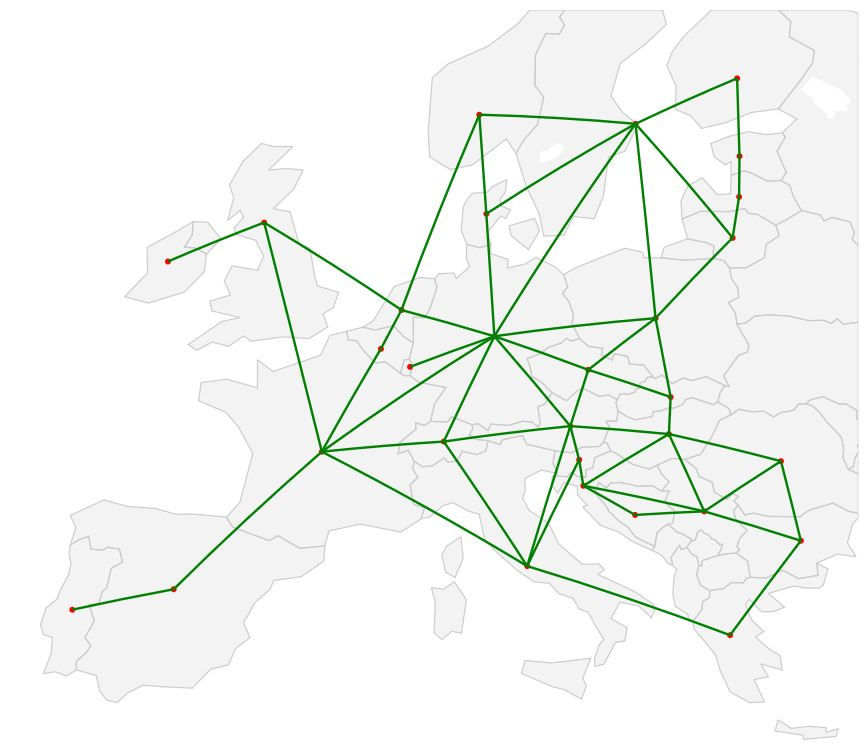
\includegraphics[width=0.95\textwidth]{./Images/network_layout}
	\caption{Network layout}
	\label{fig:network_lay}
\end{figure}
	
\section{The optimization problem}\label{sec:OptimizationProblem}


The optimization problem at hand is a simplified energy economic model of Europe, build with focus on exploring the composition of VRES (variable renewable energy sources) on a global and national scale. In the model each country is represented as a note connected to the surrounding countries through a link. Each country has three energy producing technologies available, gas, wind and solar power. A data resolution of 1 hour is used, and simulations run over an entire year. 

Following the naming convention from \cite{PyPSA_euro_30_model}, indexing the notes in the network with the variable $n$, the power generating technologies by $s$, the hours in the year by $t$ and the possible connecting power lines by $l$, the contributing variables to the objective function describing the total annualized system cost is the following: 

\begin{itemize}
	\item Hourly dispatch of energy from the given plants in the given countries $g_{n,s,t}$ with the marginal cost $o_{n,s}$.
	\item Total installed capacity of the given technologies in the given countries $G_{n,s}$ with the capital cost $c_{n,s}$.
	\item Total installed transmission capacity for all lines $F_{l}$ with the fixed annualized cost $c_{l}$.
	
\end{itemize}

The objective function for the optimization problem then becomes: 

\begin{equation}
min \left( \sum_{n,s} c_{n,s} G_{n,s} + \sum_l c_l F_l + \sum_{n,s,t} o_{n,s} g_{n,s,t} \right)
\end{equation}{}

This objective function is subject to a range of constraints ensuring realistic behavior of the system. As described in \cite{PyPSA_euro_30_model} a power balance constraint is issued to ensure stable operation of the network. These constraints force the sum of energy produced and consumed in every hour to equal zero. The hourly electricity demand at each node is described by $d_{n,t}$, the incidence matrix describing the line connections is given by $K_{n,l}$ and the hourly transmission in each line is described as $f_{l,t}$. Then the power balance constraint becomes:

\begin{equation}
\sum_s g_{n,s,t} - d_{n,t} = \sum_l K_{n,l} f_{l,t} \; \forall n,t
\end{equation}

For all conventional generators the maximum hourly dispatch of energy is limited by the installed capacity. It is important to node that for all simulations performed in this project the installed capacity is a variable. 

\begin{equation}
0\leq g_{n,s,t} \leq G_{n,s} \; \forall n,s,t
\end{equation}

The dispatch of variable renewable energy sources (wind and solar) is not only limited by the installed capacity, as availability, hence the name, is variable. Therefore the constraint for dispatch of variable renewable energy sources become:

\begin{equation}
0 \leq g_{n,s,t} \leq \overline{g}_{n,s,t} G_{n,s} \; \forall n,s,t
\end{equation}

Where $\overline{g}_{n,s,t}$ represents the normalized availability per unit capacity. 

The installed capacity is constrained by the geographical potential calculated in \cite{PypsaModel}.

\begin{equation}
0 \leq G_{n,s} \leq G_{n,s}^{max} \; \forall n,s
\end{equation}

All transmission lines in the model modelled with a controllable dispatch constrained by the fact that there must be energy conservation at each node the line is connected to. !! Something here about which lines is included !!!! . Furthermore the transmission in each line is limited by the installed transmission capacity in each line. 

\begin{equation}
|f_{l,t}| \leq F_l \; \forall l,t
\end{equation}

In the model it is possible to activate a CO2 constraint, limiting the allowed CO2 emissions for the entire energy network. As in \cite{PypsaModel} the constraint is implemented using the specific emissions $e_s$ in CO2-tonne-per-MWh of the fuel for each generator type $s$, with the efficiency $\eta_s$ and the CO2 limit $CAP_{CO_2}$. 

\begin{equation}
\sum_{n,s,t} \frac{1}{\eta_s}g_{n,s,t} e_s \leq CAP_{CO_2}
\end{equation}

The model is implemented in the open source software PyPSA \cite{Pypsa}, using much of the software presented in \cite{PypsaModel}. Optimization of the model is performed with the optimization software Gurobi \cite{Gurobi}. 

\section{Properties of the near optimal feasible space}\label{sec:properties_of_hull}

Analyzing the original optimization problem one can deduct that the feasible decision space, must be convex, as all constraints $f_i$ and the objective function $f_0$ satisfy equation \vref{eq:convex_requirement}, and therefore must be convex \cite{ConvexOpimization}. 

\begin{equation}\label{eq:convex_requirement}
f_i(\alpha x + \beta y) \leq \alpha f_i(x) + \beta f_i(y) \; \forall \; x, y \in \mathbb{R}^n and  \; \alpha, \beta \in \mathbb{R}
\end{equation}

Furthermore, when all variables are bounded; hourly production by the power balance constraint and installed capacity by geographical potential, the feasible decision space is not only convex but also closed. If the geographical potential constraint is excluded the feasible decision space becomes an open convex space as illustrated on \vref{fig:sketch_feasable_space}, this does however not have any immediate consequences, as the objective function increases as one moves in the open direction of the space. 

\begin{figure}[ht]
	\centering
	\incfig{Feasible-space}
	\caption{A sketch of a one dimensional feasible space with MGA constraint }
	\label{fig:sketch_feasable_space}
\end{figure}

\begin{equation}
W = \{ \vec{x}\in \mathbb{R}^d | f_i(x) \geq 0 \}
\end{equation}
!!! This is not completly right !!! 


It is important to note that the variables $\vec{x}$ that defines the decision space in the original solutions are, all hourly technology dispatches $g$, all installed capacities $G$ and all installed line capacities $F$. 

\begin{equation}
\vec{x} = \{g_{n,s,t} \wedge G_{n,s} \wedge F_l \; \forall \; n,s,t,l \}
\end{equation}

Therefore, the dimensionality, of the decision space must be given by the number of nodes in network $n$ for every technology $s$ for every hour $t$, plus the number of nodes $n$ times technologies $s$ and finally the number of lines $l$  \vref{eq:dimentionality}.

\begin{equation}\label{eq:dimentionality}
d = n\cdot s \cdot t + n\cdot s + l
\end{equation}


In the case of the reference model used in this project that gives 
$ 30 \cdot 3 \cdot 8765 + 30 \cdot 3 + 90 = 789030$ 
!!! number of lines is a guestimate!!

The true dimensionality might be lower, as some variables do have strong corelations. 

\subsection{Sub space}

As the dimensionality of the decision space is very large, and therefore becomes very unhandy to work with, it makes sense to look at a subspace of lower dimensionality. One could choose to ignore the hourly dispatch of energy from the individual generators, hereby reducing the dimensionaly by a substantial amount. 

\begin{equation}
d^* = n\cdot s + l
\end{equation}

In that case the dimensionality would only be $d^* = 30\cdot 3 + 90 = 180$. 

The subspace would then be given by:

\begin{equation}
W^* = \{\vec{x}^* \in \mathbb{R}^{d^*} |    \}
\end{equation}

The set $W^*$ therefore includes information about installed capacities of all technologies and transmission lines. Since plant operation, is not the focus of this project, but rather distribution of capacities,  the subspace $W^*$ still provides the information of interest, despite its much lower dimensionality. 

\subsubsection{Further reduction}
If desired it is possible to further reduce dimensionality, by sacrificing all spatial information.

\begin{equation}
x^{**} = \{\sum_n G_{n,s} \forall n,s  \}
\end{equation} 

\begin{equation}
d^{**} = s
\end{equation}

\begin{equation}
W^{**} = \{\vec{x}^{**} \in \mathbb{R}^{d^{**}} |    \}
\end{equation}



\section{Modeling to Generate Alternatives (MGA)}\label{sec:MGA}
In this section the basic principles of MGA will be explained together with the benefits and challenges this technique introduces. 

\subsection{Motivation for using MGA}

In the field of mathematical modeling, the scientist aim to produce models representing physical systems as realistically as possible. However, some degree of uncertainty in the models is inevitable as model fidelity is limited by a range of factors including: numeric precision, uncertainty of data, model resolution etc. Modeling of energy systems is a field especially prone to large model uncertainties, deriving not only from lack of fidelity, but from factors such as unmodeled objectives and structural uncertainty \cite{DeCarolis_MGA}. 

The MGA approach was first introduced in 1982 by Brill et al. \cite{Brill_MGA_1982}, in the field of operations research/management science. This is a field where unmodeled objectives and structural uncertainty, are highly influential. 

!! CITATION !!
The basic insight can be
summarized as follows: Because it is not possible to develop a complete
mathematical representation of complex public planning problems,
structural uncertainty in optimization models will always exist. As a
result, the ideal solution is more likely to be located within the model's
inferior region rather than at a single optimal point or along the noninferior frontier (Brill, 1979)

Policy makers often have strong concerns outside the scope of most models
(e.g., political feasibility, permitting and regulation, and timing of
action), which implies that feasible, suboptimal solutions may be
preferable for reasons that are difficult to quantify in energy economy
optimization models.

The purpose of MGA is to efficiently search the feasible
region surrounding the optimal solution to generate alternative
solutions that are maximally different. !!!

\subsection{Technical explanation of MGA HSJ}

The MGA technique was first introduced in 1982 by Brill et. al in the article \cite{Brill_MGA_1982} and later rediscovered by DeCarolis in \cite{DeCarolis_MGA} for use in energy system optimization. The tecnique lets the user search the near optimal feasible decision space for an optimization problem such as the one addressed in this project described in \ref{sec:OptimizationProblem}. 

In section \ref{sec:OptimizationProblem} a series of constraints bounding the network model is listed. Together these constraints form a feasible region that can be described as a convex set in a $d$ dimensional space. Where d is the number of variables in the model. The feasible set is convex as all bounding constraints are linear. The fact that linear constraints form a convex set is shown in \cite{ConvexOpimization}. The MGA technique introduces yet another constraint limiting the size of this convex set even further by limiting the objective function value of all feasible points to be within a certain range of the optimal solution. The goal of the MGA technique is to explore a finite set of alternative solutions located within this convex set. 

In the orginal articel by Brill et. al \cite{Brill_MGA_1982} the HSJ MGA technique is descrbed with the following steps. 

(1) obtain an initial optimal solution for the problem at hand; (2) define a target value for the objective function by adding a user specified amount of slack to the value of the objective function in the initial solution (3) introduce the constraint limiting the objective function to surpass this target value, to the model (4) formulate a new objective function that seeks to minimize the sum of decision variables that had non zero values in the previous solution of the problem (5) iterate the reformulated problem, updating the objective function every time (6) terminate the optimization when the new solution is similar to or close to any previously found solution. Step 3 and 4 was described mathematically in \cite{Brill_MGA_1982} as follows:

\begin{equation}
\begin{split}
Minimize :&  p = \sum_{k \in K} x_k \\
Subject to :&  f_j(\vec{x}) \leq T_j \forall j  \vec{x}\in X
\end{split}
\end{equation}

In this formulation $k$ represents the variable indices for the variables with nonzero values in the previous solution, $j$ is the objective function indices if multiple objective functions exists, $f_j(\vec{x})$ is the evaluation of the $j$'th objective function and $T_j$ is the target value specified for the particular objective function. In the formulation of the constraint $\vec{x}\in X$ specifies that all previously defined constraints still applies as all new solutions $\vec{x}$ must be a part of the set of feasible solution vectors from the original formulation $X$.

How the new objective function precisely is formulated and which variables to include is discussed in \cite{DECAROLIS2016}, where two alternative approaches of defining the new objective function is presented. One approach suggest giving all nonzero variables from the last iteration a weight of 1 in the new objective function. This approach does not consider weight from previous iterations. However, the second approach suggests adding on to the coefficient with a factor of +1 for every time one variable has appeared with nonzero in a row, hereby further increasing the intended to reduce the use of that specific technology. This 



\subsection{Other MGA approaches}

\section{Novel MGA approach}

In this section a novel approach towards MGA optimization of energy networks will be presented. Based on the same concepts as presented in \ref{sec:MGA} this method seeks to explore not only a few alternative solutions from the decision space, but the entire decision space. Hereby an in depth knowledge of the possible solution is obtained providing insight in the distribution of alternative solutions.

An important feature about the method developed is that it can be used for any dimensional decision space. 

The method developed can be divided into two phases. In the first phase, the shape of the feasible near optimal decision space is found, and in the second phase relevant data is extracted from the found space. 

\subsection{Decision space mapping}
As explained in section \vref{sec:properties_of_hull}, the near optimal feasible space will always be convex, and can either be closed or not. However, when the MGA constraint from equation \vref{eq:MGA_constraint} is introduced the space will be closed. 

\begin{equation}\label{eq:MGA_constraint}
f(\vec{x}) \leqslant f(\vec{x}^*) \cdot (1+\epsilon)
\end{equation}

As we now have a closed convex space, it now is possible to explore the shape of this convex set. Assuming that all constraints used including the MGA constraint is linear, the convex set must be a polyhedral and therefore it is possible to define the shape of this set with a finite number of vertexes. !!! This might not be the case for CO2 constraint!!!! \\

However, finding these vertices is no trivial task. In the method developed, all solutions found, that lie within the near optimal feasible space is treated as a point in that space. Furthermore, the possibility of letting the objective function search in a given direction in the decision space is utilized, by replacing the original objective function to an objective function on the from presented in \vref{eq:objective_func_face_normal}.

\begin{equation}\label{eq:objective_func_face_normal}
Minimize \; p = \vec{n}_i\vec{x}
\end{equation}

Where $\vec{n}_i$ is the $i$'th normal vector. 


The method proposed here will use the following steps to approximately find all vertices. 

\begin{enumerate}
	\item Find initial solution
	\item Add MGA constraint
	\item Maximize and minimize all variables
	\item Based on these points define a convex hull, and define all face normals
	\item Iterate over each face normal and change objective function to \vref{eq:objective_func_face_normal}
	\item Add the newly found points to list of points and define new hull and its face normals 
	\item Repeat step 5 and 6 until the size of the convex hull converges 
\end{enumerate}

The convergence criteria used in this project is that the hull size must not increase by more than 2\% in two consecutive iterations. 

The result of following these steps is a list of points defining a hull in $d$ dimensional space, however this on its own does not provide much usefull information. To gain any knowledge about the network being analysed on must follow the steps provided in part two of this method. 

\subsection{Hull fill}










\subsection{Pseudo code}

\begin{itemize}[label={}]
	\item Solve network subject to regular constraints and with original objective function
	\item Add MGA constraint !Equation number
	\item while $\epsilon>tol$
	\begin{itemize}[label={}]
		\item If first loop
		\begin{itemize}[label={}]
			\item directions = max and min all variables
		\end{itemize}
		\item Else
		\begin{itemize}[label={}]
			\item directions = normals to hull faces
		\end{itemize}
		\item for direction in directions
		\begin{itemize}[label={}]
			\item objective function = direction[i] * variable[i]
			\item point on convex hull += solve problem subject to objective function
		\end{itemize}
		\item hull = ConvexHull ( points on convex hull)
		\item $epsilon$ = new hull volume - old hull volume / hull volume
	\end{itemize}
	\item Evenly distribute points in hull 
	\item Plot histogram using evenly distributed points. 
\end{itemize}

\section{Implementation and utilization of parallel programming}







%\clearpage

\chapter{Model}\label{chap:model}

The purpose of this section is to present the techno-economic model used in this project. In the previous chapter, the mathematical framework of a techno-economic model was presented, and in this chapter, the physical interpretations of the equations making the model will be discussed. Furthermore, all the time-series and cost data used in the model will be presented. The model used in this project is heavily inspired by the work performed in \cite{PyPSA_euro_30_model}. 

\section{Topology}
The model used in this project is based on the work presented in \cite{PyPSA_euro_30_model}, where a model spanning the electricity grid of 30 European countries is formulated as a techno-economic linear optimization problem. Countries included in the model are the EU-28 countries not including Cyprus and Malta, instead of including Norway, Switzerland, Serbia, and Bosnia and Herzegovina.

The topology of the network presented in Figure \ref{fig:network_lay}, is such that each node represents a country and the links represent international HVDC or HVAC links. The links included are based on currently installed international transmission lines. 


\begin{figure}[h]\centering
	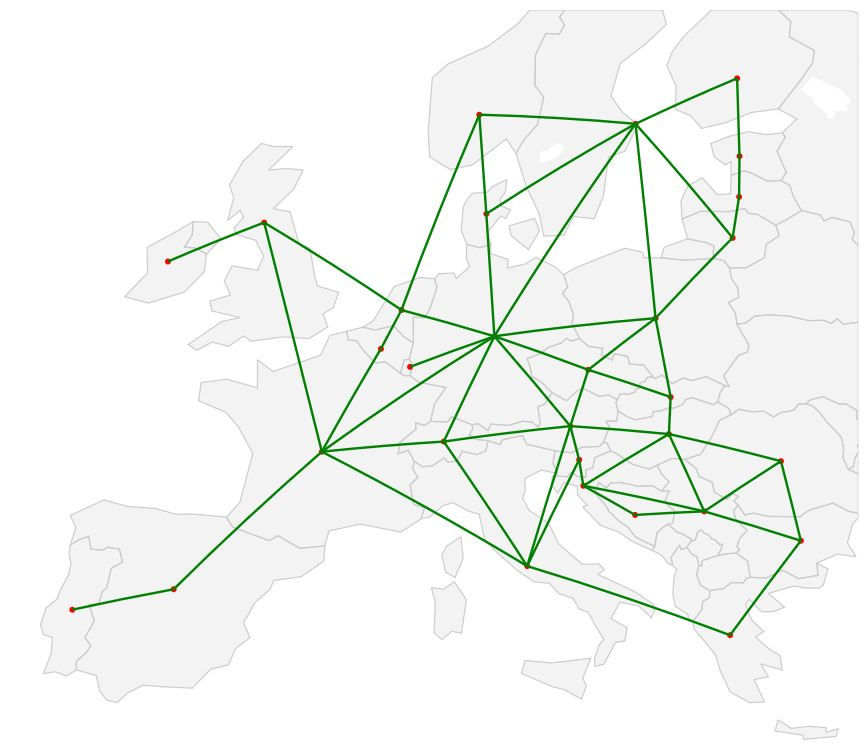
\includegraphics[width=0.75\textwidth]{./Images/network_layout}
	\caption{This figure shows the topology of the techno-economic model used in this project. Green lines represent transmission lines and red dots present the location of centroid of all countries included in the model.}
	\label{fig:network_lay}
\end{figure}


All model input parameters are based on 2011 values as this is the earliest year with all data available. The temporal resolution of the model is hourly, with all simulations spanning a full year. Technology costs are all valued in 2011 Euros. 

\section{Energy production}

Each node in the network, has energy-producing technologies available, with initial capacities being zero. The available energy-producing technologies used in this project: Onshore wind, offshore wind, solar PV and open-cycle gas turbines (OCGT). In the model, all technology capacities are expandable limited only be the geographical potential. 

The geographical potentials used are calculated following the work of  \cite{PyPSA_euro_30_model}. In the calculation of geographical potential, the potential available area suited for either onshore wind, offshore wind, and solar PV, must first be defined. These areas were found by allowing certain technologies to be installed only in areas with certain land-use types. Hereby restricting onshore wind farms from being installed in cities and solar PV plants from being installed in forests etc. The placement of offshore wind farms was restricted to areas with a water depth of less than 50m. Furthermore, all nature reserves were excluded from potential areas. As competing land use and likely public acceptance issues will occur, the found potential areas are set to bee only 20\% of the found area for onshore and offshore wind and only 1\% for solar PV. 
Assuming a maximum nominal installation density of 10 $MW/km^2$ for offshore and onshore wind power, and 145 $MW/km^2$ for solar PV \cite{PyPSA_euro_30_model}, it is possible to calculate the geographical potential for the three technologies all across Europe. 

The hourly energy production of all variable renewable energy sources is limited by the production potential given by the weather. Following \cite{PyPSA_euro_30_model}, the availability was calculated using historical weather data for 2011 from \cite{ClimateForecastSystem} with a spatial resolution of 40x40 km and hourly temporal resolution. The weather data is first converted to generation potentials for each 40x40 km cell using the REatlas software \cite{ANDRESEN20151074}, and then the national hourly means are found. The mean capacity factor for wind and solar power is presented in Figure \ref{fig:capacity_factor}.


\begin{figure}[h]\centerfloat
	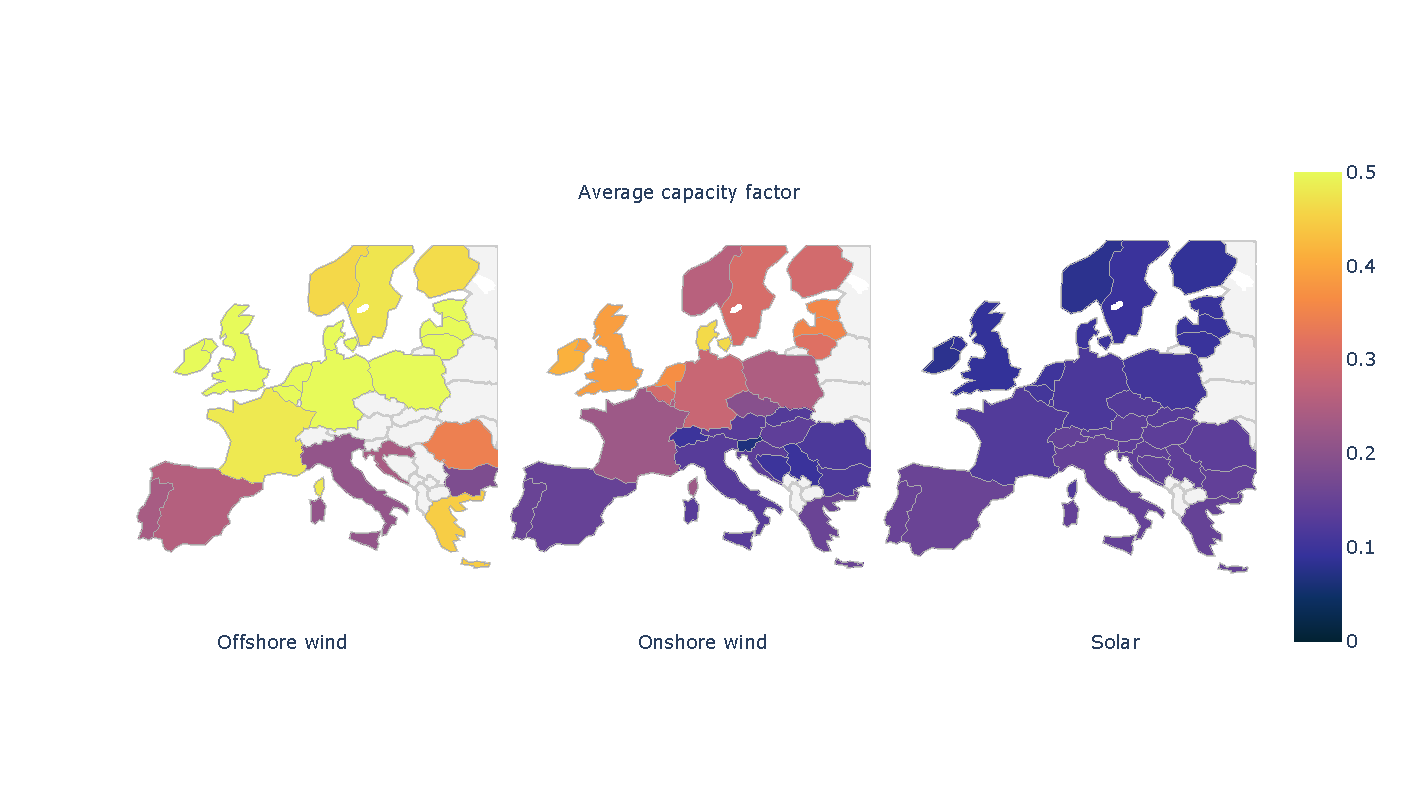
\includegraphics[width=1.3\textwidth]{./Images/wind_availability}
	\caption{The figure shows the average generation potential of wind turbines and solar PV plants, in the individual countries included in the model.  }
	\label{fig:capacity_factor}
\end{figure}



The dispatchable energy sources available in all countries are chosen to be open-cycle gas turbines (OCGT), as they have high flexibility and good load following capabilities, therefore making them suitable as a backup generator in a highly decarbonized scenario. They do however not necessarily produce realistic results when used in scenarios with low decarbonization, as other plant types such as conventional coal-powered combined heat and power perform better in these cases. The capacities and energy generation of the gas turbines are contrary to the variable renewable energy sources, not limited by geographical or generation potentials. They are, however, limited by the maximum allowable $\text{CO}_2$ emission. The $\text{CO}_2$ emission intensity of the open cycle gas turbine is 0.19 t/MW \cite{PyPSA_euro_30_model}. In this project, the $\text{CO}_2$ constraint will always be calculated as a percentage reduction in emission compared to a scenario run on the same model with the same parameters without any constraint on $\text{CO}_2$ emission. 

In countries located on the coast both onshore and offshore wind turbines are available. The capacity of these two types of wind power is however treated as one single variable in all simulations performed in this project. 

In all simulations, the capacities of all energy generators are initially set to be zero, with the capability to be expanded until geographical potentials or $\text{CO}_2$ constraints, limits further expansion. The cost of expanding capacities is calculated as annualized cost, given as the annualized investment cost plus fixed annual operations and maintenance cost. The annualized investment cost is calculated by multiplying the annuity factor (Equation \ref{eq:annuity}) by the investment cost. 

\begin{equation}\label{eq:annuity}
a = \frac{r}{1 - \frac{1}{(1+r)^n}}
\end{equation}

Where $r$ is the discount rate, and $n$ is the expected lifetime of the given technology. In this project a discount rate of 7\% \cite{PyPSA_euro_30_model} is used. The lifetime of the individual technologies are listed in Table \ref{tab:cost_data}. All cost data are based on the 2030 values presented in \cite{Schroder2013Current}.

\begin{table}[]
	\begin{tabular}{l|llll}
		Technology      & \makecell[c]{Investement \\ {[}€/MW{]}}    & \makecell[c]{Fixed O\&M \\ {[}€/kW/year{]}} & \makecell[c]{Marginal cost \\ {[}€/MWh{]}}    & \makecell[c]{lifetime \\ {[}years{]}} \\ \hline
		Onshore Wind    &       1182          &   35      &   0.015       &   25       \\
		Offshore Wind    &        2506        &    80        &    0.02        &    25        \\
		Solar PV           &       600            &   25      &   0.01        &   25       \\
		OCGT               &       400            &   15      &   58.4        &   30      \\
		Transmission    &   \makecell[l]{ 400 €/MW km \\ +150000€ pr line}  & 2\% & 0         &   40 
	\end{tabular}
	\caption{Generator parameters are based on the values from \cite{Schroder2013Current}, and transmission parameters are based on the work presented in \cite{HAGSPIEL2014654}.}
	\label{tab:cost_data}
\end{table}

\section{Energy demand}
The data for the hourly electricity demand found in the European Network of Transmission System Operators data portal is used as energy demand \cite{ENTSO-E}. The data has a resolution of one hour and is provided for all countries included in the model. In Figure \ref{fig:demand}, the summarized demand for the entire year for the individual countries is shown. A total of $3152$TWh of energy was consumed by the countries combined in 2011. 

\begin{figure}[h]\center 
	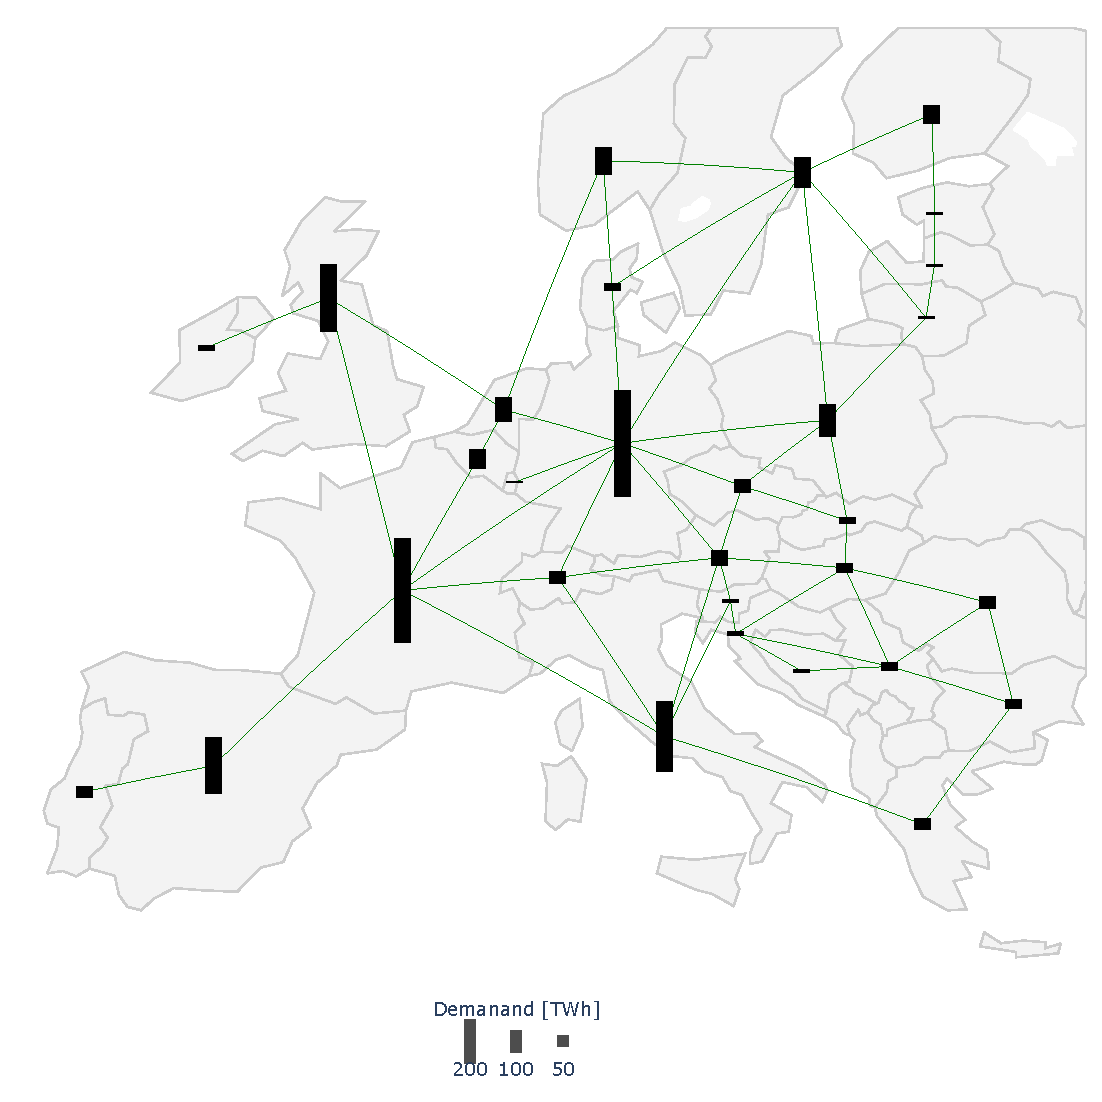
\includegraphics[width=.8\textwidth]{./Images/Demand}
	\caption{The figure shows the total electricity demand of the individual countries during an entire year. }
	\label{fig:demand}
\end{figure}

\section{Energy transmission}
In the model used in this project, all transmission lines are treated as transport models with a coupled source and sink, only constrained by energy conservation at each connecting node. Transmission loss is thereby not considered. This approximation is assumed to be acceptable as most international transmission lines already are, or probably will be in the near future, controllable point-to-point high voltage direct current (HVDC) lines. 

Line capacities initially start as zero, and can then be expanded if found feasible in the optimization, with no constraint on the maximum allowable capacity. The investment cost of line capacity is calculated as a cost pr MWkm plus an additional cost for a high voltage AC to DC converter pair. The price of a high voltage AC to DC converter pair is set to be 150000€ regardless of line capacity \cite{HAGSPIEL2014654}. 

The length of each line is set as the distance between the centroids of each connecting country plus an additional 25\%. The extra 25\% is added to the line length as competitive land use and public acceptance issues will prohibit lines from being placed in optimal positions. 

Furthermore, to satisfy n-1 security the price is adjusted with a factor of $1.5$, to account for the extra installed capacity needed, as shown in \cite{PyPSA_euro_30_model}. 

\begin{equation}
c_l = \left( L\cdot I_s \cdot 1.25+150000 \right) 1.5 \cdot 1.02 \cdot a
\end{equation}

%1.25 = 25\% extra length due to land use competition. 
%150000  Price of DC converter pair
%1.5 = n-1 security 
%1.02 = 2\% FOM (fixed operations and maintenance cost)
%a = annuity 



\section{Utilization of parallel programming and cluster computing}
As the MGA approach described in Section \ref{sec:Novel_MGA} requires a high number of similar optimizations to be performed only with slightly changed objective functions, it is possible to achieve a great performance boost, by utilizing parallel programming and cluster computing.

The model used in this project is implemented in the open-source tool PyPSA \cite{Pypsa}, build for the programming language Python. The individual optimizations of the model are done with the optimization tool Gurobi \cite{Gurobi}. The Gurobi solver is capable of using several computing cores to speed up the process of optimizing the model. Allowing Gurobi to use two cores, it is possible to find an optimal solution to the techno-economic model used in this project in approximately 20 minutes. As the MGA method presented in this project requires several optimizations of the problem, with a changing objective function, it is possible to reduce the computation time drastically by utilizing parallel programming. 

Using the Python framework  Multiprocessing \cite{Multiprocessing}, the MGA method presented in this project was implemented, capable of performing several optimizations at once. Using the PRIME compute cluster \cite{Prime}, it was possible to perform 16 parallel optimizations on the 32 core compute nodes, reducing the time needed per MGA study drastically. 
The Prime compute cluster \cite{Prime}, has 17 compute nodes with 24-36 cores available each operating at roughly 3 GHz, giving a total of 538 cores. Performing an MGA study requires anything in the range of 100-2000 optimizations of the model, each one requiring two cores for twenty minutes. Using a single compute node with 32 cores a single MGA study can be performed in a few hours up to two days, depending on the complexity of the problem. 




\chapter{Results}
Several computational experiments have been performed to analyze the performance of the novel MGA approach developed in this project, and to study the techno-economic model of Europe presented. Initially the results of a study performing regular optimization of the techno-economic model of Europe is presented, providing a basic insight in the techno-economic model used. Knowing the optimal solutions to the optimization problem, the results of a study implementing the novel MGA method presented in this project, are presented. This study seeks to investigate how the installed capacities of the different technologies are distributed across all near optimal feasible solution to the problem.
Yet another MGA study is performed, analyzing the interplay between energy production in south and north Europe. This study also seeks to investigate the limitations of the MGA algorithm, in terms of the maximum allowable variables included in the decision space considered by the MGA algorithm. 
In order to compare the usefulness of the novel MGA approach developed in this project, a study comparing the novel MGA approach with previously presented MGA approaches have been performed. The results of this study will be presented, highlighting benefits and disadvantages of a total of four different MGA approaches including the one presented in this project. 


\section{Optimal solutions}
Before any MGA studies are performed, the baseline performance of the techno-economic model must be established. This is done by performing classic optimization of the models in order to find the optimal solutions. 

Initially the model is optimized without introducing any $\text{CO}_2$ constraints, in order to establish a baseline for $\text{CO}_2$ emissions. The baseline $\text{CO}_2$ emissions measured in tonnes per year, acts as the reference for $\text{CO}_2$ reductions in other scenarios. It is important to perform this study as real world numbers on $\text{CO}_2$ emissions doesn't necessarily compare to the numbers found using this specific model. This is due to the fact that the model used in this project simplifies the complex energy grid of Europe by a great deal, hereby introducing a lot of uncertainty. It is therefore relevant to compare the performance of the model used in this project to the performance of the actual energy system. 

When the optimal solution for the model with no $\text{CO}_2$ constraints is found, a range of optimizations are performed with altering $\text{CO}_2$ constraints. The allowable $\text{CO}_2$ emissions are calculated as a percentage of the emission of the base scenario. A total of three $\text{CO}_2$ reduction levels was chosen to investigate being 50\%, 80\% and 95\% reduction compared to the base scenario. The objective of performing these optimizations is to investigate the effect of the $\text{CO}_2$ constraint on the model, before performing any MGA studies. 

%Before starting any MGA studies, it is important to investigate and understand the optimal solution of the problem at hand. In this section, the found optimal solutions of the model will be presented. A range of $\text{CO}_2$ constraints have been investigated, and as the $\text{CO}_2$ constraint is altered a new optimal solution is found, therefore four optimal solutions representing a business as usual scenario, a 50\% $\text{CO}_2$ reduction, a 80\% $\text{CO}_2$ reduction and a 95\% $\text{CO}_2$ reduction scenario will be presented. 

\begin{figure}[h]\centering
\begin{subfigure}{1\textwidth}
	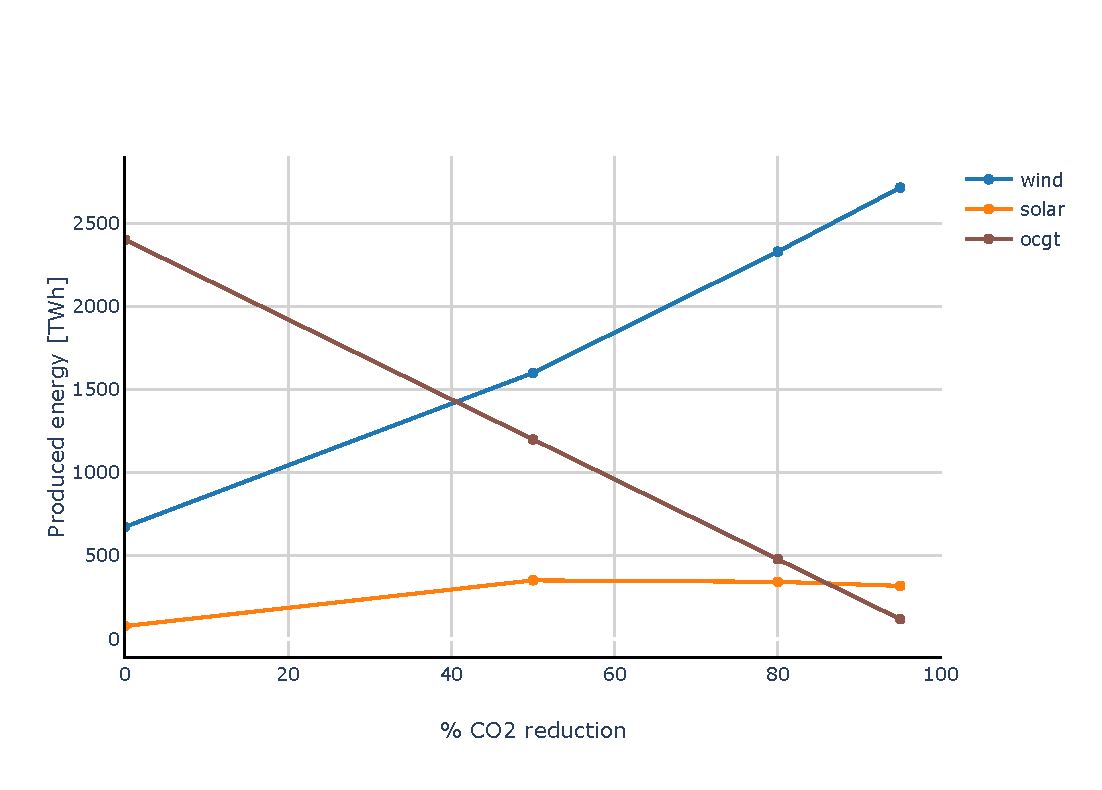
\includegraphics[width=.9\textwidth,trim={0 0cm 0cm 2.8cm},clip]{./Images/optimal_solutions_summary_production}
	\caption{}
	\label{fig:Optimal_Solutions_produc}
	\end{subfigure}%
\vspace{-10pt}
\begin{subfigure}{1\textwidth}
	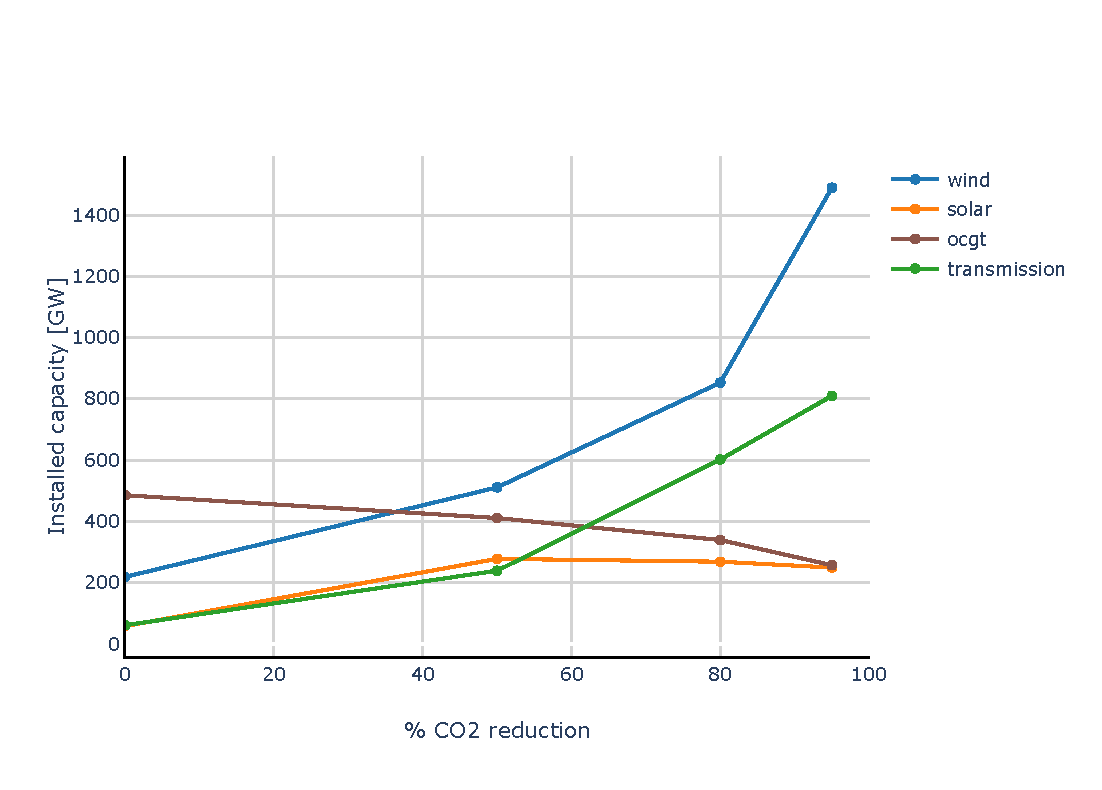
\includegraphics[width=1\textwidth,trim={0 0cm 0cm 2.8cm},clip]{./Images/optimal_solutions_summary}
	\caption{}
	\label{fig:Optimal_Solutions_summary}
\end{subfigure}%
\caption{Figure (a) shows the total amount of produced energy by the individual technologies during an entire year, for the four optimal solutions with different reductions in CO2 emissions. On figure (b) a summary of the total installed technology capacity versus \% $\text{CO}_2$ reduction for the four optimal solutions is presented.}
\label{fig:Optimal_Solutions_summary_both}
\end{figure}

\begin{table}[h]
	\begin{tabular}{lr|llll}
		Technology      & & Business as usual & 50\% $\text{CO}_2$  & 80\% $\text{CO}_2$  & 95\% $\text{CO}_2$  \\ \hline
	wind &[GW] & 219.1 & 511.2 & 853.3 & 1489.5 \\
	Solar &[GW]& 58.6 & 278.0 & 268.78 & 249.6 \\
	OCGT &[GW]& 485.5 & 411.2 & 339.4 & 257.2 \\
	Transmission &[GW]& 61.4 & 239.5 & 602.3 & 810.1 \\
	Gini coefficient & & 0.11 & 0.20 & 0.44 & 0.59 \\
	$\text{CO}_2$ emission &[MT] & 1151.9 & 576.0 & 230.4 & 57.6 \\
	Objective value &[1e9\euro] & 200.7 & 212.8 & 256.5 & 358.1 \\         
	\end{tabular}
	\caption{Key data from the four optimal solutions are presented.}
	\label{tab:Optimal_Solutions_summary}
\end{table}

On figure \ref{fig:Optimal_Solutions_summary}, the summarized technology capacities are presented, showing how the two $\text{CO}_2$ neutral energy sources increase as the $\text{CO}_2$ constraint is tightened. It is important to note how the installed wind capacity increases rapidly compared to solar PV that levels out, as the $\text{CO}_2$ reduction reaches the higher percentages. This could indicate that any further solar PV capacity would primarily generate surplus energy, as long as no storage technologies are implemented. Studies have previously shown that solar PV is highly dependent on short term storage if it is to be utilized on a larger scale \cite{rasmussen2011a} \cite{VICTORIA2019111977}. This is due to the high daily fluctuations in energy production from solar PV and therefore solar PV has a great synergy with short term storage technologies. 

Figure \ref{fig:Optimal_Solutions_summary} further shows that a wind solar mix of approximately 80\% wind and 20\% solar PV is desirable, when no storage solutions are implemented, if +90\% $\text{CO}_2$ reduction should be achieved. This complies very well with the results presented in \cite{rasmussen2011a}, where a study on the optimal wind and solar mix for Europe is performed. 

Comparing the produced energy in the four scenarios presented on figure \ref{fig:Optimal_Solutions_produc} with the installed capacities from figure \ref{fig:Optimal_Solutions}, it is seen how the energy produced by gas turbines drops drastically compared to the gas turbine capacity as $\text{CO}_2$ emissions are reduced. This means that every GW of installed OCGT capacity produces less energy in the scenarios with high $\text{CO}_2$ reduction. Instead of acting as primary energy source the gas turbines changes role and instead acts as backup capacity. The amount of produced energy from wind turbines compared to the installed capacity also seems to decrees when the $\text{CO}_2$ reduction increases above 80\%. This could indicate that after this point, additional installed wind capacity generates more surplus then previously installed capacity. 


The Gini coefficients for the four scenarios is presented in table \ref{tab:Optimal_Solutions_summary} and on figure \ref{fig:Gini}. The Gini coefficient expresses the equality in production versus consumption for the four scenarios. A low Gini coefficient indicates that energy is being produced locally and opposite, a high Gini coefficient indicates that energy is being produced away from where it is needed. The Gini coefficients of the four optimal solutions appears to increase, together with the capacity of wind and solar power, as the $\text{CO}_2$ constraint is tightened. This could suggest that it is beneficial to install wind and solar power in countries with good wind and solar profiles and then transmit the energy to countries with less favorable wind and solar profiles. Analyzing the average capacity factors for wind power on figure \ref{fig:capacity_factor}, it is seen that higher capacity factors are common in northern countries. This corespondents very well with where the large capacities of wind are placed in the optimal solutions subject to high $\text{CO}_2$ constraints presented on figure \ref{fig:Optimal_Solutions}c and \ref{fig:Optimal_Solutions}d. Comparing the installed capacities presented on figure \ref{fig:Optimal_Solutions} with the total demand of the individual countries presented in figure \ref{fig:demand}, it is clearly seen that as $\text{CO}_2$ emissions are reduced, the installed capacities moves further and further away from the countries with the largest demands. 

\begin{figure}[h]\centerfloat
	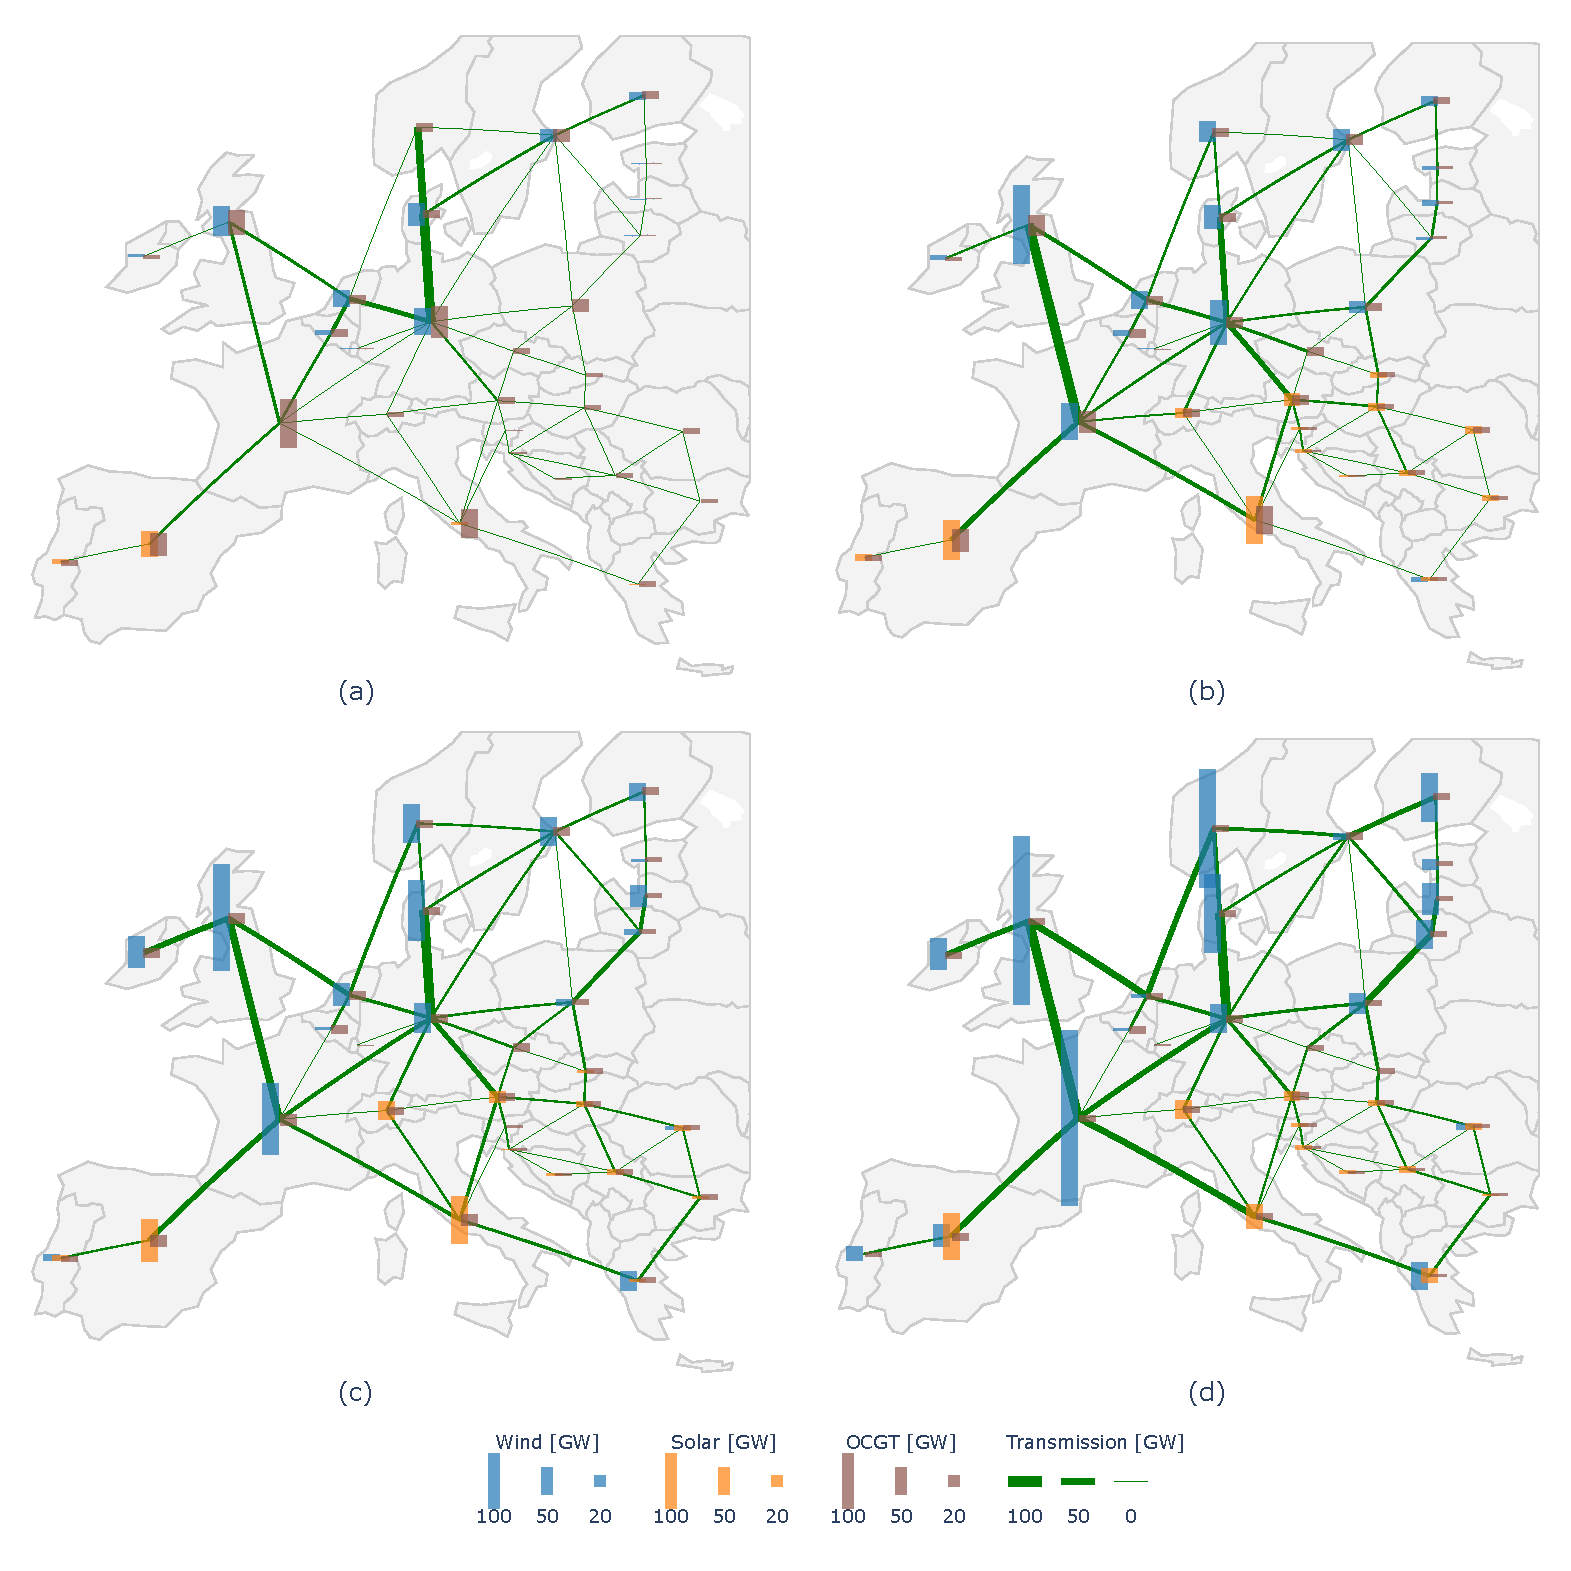
\includegraphics[width=1.1\textwidth]{./Images/Optimal_solutions}
	\caption{The figure presents the layout of technology capacities of all four optimal solutions. On figure (a) the business as usual scenario is presented, (b) shows data for the scenario with 50\% CO2 reduction, (c) 80\% reduction and (d) 95\% reduction in CO2 emissions.}
	\label{fig:Optimal_Solutions}
\end{figure}

\subsection{Business as usual}
In the business as usual scenario, seen on figure \ref{fig:Optimal_Solutions}a, where no constraint on the $\text{CO}_2$ emission is implemented, energy is primarily supplied by gas turbines as expected. Any significant capacities of variable renewable energy sources is only implemented in countries where the price of energy produced from such technologies can compete with the price of energy from gas turbines. Analyzing figure \ref{fig:capacity_factor} it is found that wind energy is favorable in the northern countries and solar energy only becomes favorable in the most southern countries, in this case Spain and Portugal. 
Furthermore, the energy generation is spread, fairly even across the network, thereby requiring less transmission capacities, and thereby also resulting in a fairly low Gini coefficient of 0.11. In this scenario transmission is purely installed between countries with significant shares of VRES. 

The $\text{CO}_2$ emission in the base scenario without $\text{CO}_2$ constraints was found to be 1151.9 MT $\text{CO}_2$/year, which complies reasonably well with the 2011 $\text{CO}_2$ emission for the EU-28 countries energy sector, found by the European Environment Agency (EEA) to be 1517.3 MT $\text{CO}_2$/year \cite{eea_co2_emission}. Although the numbers are off by some hundred MT $\text{CO}_2$/year, and the numbers from EEA only represent the EU-28 countries, this comparison can conclude that the model used in this project, despite its coarse spatial resolution and small number of included technologies, is capable of producing results with an acceptable accuracy. 


\subsection{Reduced $\text{CO}_2$ emission scenarios}

The distribution of installed capacities of the scenarios with reduced $\text{CO}_2$ emissions are presented on figure \ref{fig:Optimal_Solutions}b, c and d, with respectively 50, 80 and 95\% $\text{CO}_2$ reduction. All three scenarios implements wind energy in northern Europe and implements large amounts of transmission capacity between all countries with high shares of wind power. OCGT capacity appears to be evenly spread across the countries. Significant shares of solar power is only implemented in southern Europe, and even with a $\text{CO}_2$ reduction of 95\%, the most northern country to install solar power is Austria. 
As the $\text{CO}_2$ constraint is tightened, the Gini coefficient increases, as the countries with favorable conditions for solar and wind power, simply increases their capacity of these technologies. Whereas, technology capacities in less favorable countries stay unaffected. 

Looking at the scenario costs in table \ref{tab:Optimal_Solutions_summary}, it is seen that as the $\text{CO}_2$ constraint is tightened, the cost increases rapidly. From the business as usual scenario to the scenario with a 50\% reduction there is only an increase in price of 6\%. When the $\text{CO}_2$ emissions is to be reduced beyond this point, price increases rapidly, and to achieve a reduction of 95\% the cost almost double, having increased with 78\%, compared to the business as usual scenario. This also complies with the data shown in figure \ref{fig:Optimal_Solutions_summary_both}, where it can be seen that total installed production capacity increases, even though the energy demand stays the same. These result are very much in line with the results found in \cite{Gorm_Surplus}, where surplus electricity is investigated in scenarios with large shares of variable renewable energy sources. 

\section{MGA study of four dimensional decision space}\label{sec:4D}
The objective of this experiment is to document the performance of the techniques developed in this project, by studying the techno-economic model presented in chapter \ref{chap:model}. Focus is placed on the relevance/usability of the data extracted from the model using the newly developed technique, as well as shear performance measured in computation time. The experiment will explore the interplay between variable renewable energy sources and transmission on an international level spanning all countries in the model. 

In this experiment the decision space is reduced to just four dimensions by grouping the decision variables as explained in section \ref{sec:dim_reduction}. The four variables in the new decision space is the total amount of installed gas turbine (OCGT) capacity, wind turbine capacity, solar pv capacity and the total installed transmission capacity. Using a low dimensional space allows for a thorough exploration of the feasible space as a lower dimensional decision space, needs fewer computations per study, thereby reducing computation time. 

As a thorough exploration of the near optimal feasible space is desired, to evaluate the performance of the technique, combined with a desire to learn more about the features of the near optimal feasible space, a range of MGA studies is performed with varying parameters. 
For every single MGA exploration there are two parameters that can be altered. These are the amount of reduction in $\text{CO}_2$ emission compared to the base model, and the amount of MGA slack used. For this experiment it was chosen to iterate over both of these variables exploring $\text{CO}_2$ reductions of 0, 50, 80 and 95\%, and MGA slacks of 1, 2, 5, and 10\%. This means that a total of 16 MGA studies is to be performed. 

Even though it was established that multiplicity of sampled points has a large effect on the results, when a high dimensional space is reduced to one of much lower dimension, it has not been accounted for in this study, due to the added computing time needed. 


%- Very large range of possible configurations for VRES and Transmisison, OCGT more limited
%- OCGT has sharp lower limit
%- Solar power can be ommitted if desired
%- Tighter CO2 caps results in larger investement flexibility. As Fabian \cite{Fabian_MGA} unlike Price \cite{MGA_Price}

%In the first MGA study performed it was chosen to explore a four dimensional near optimal feasible space, with the four dimensions being total installed ocgt capacity, total installed wind capacity, total installed solar PV capacity and total installed transmission capacity. 

\begin{figure}[p]\centerfloat
	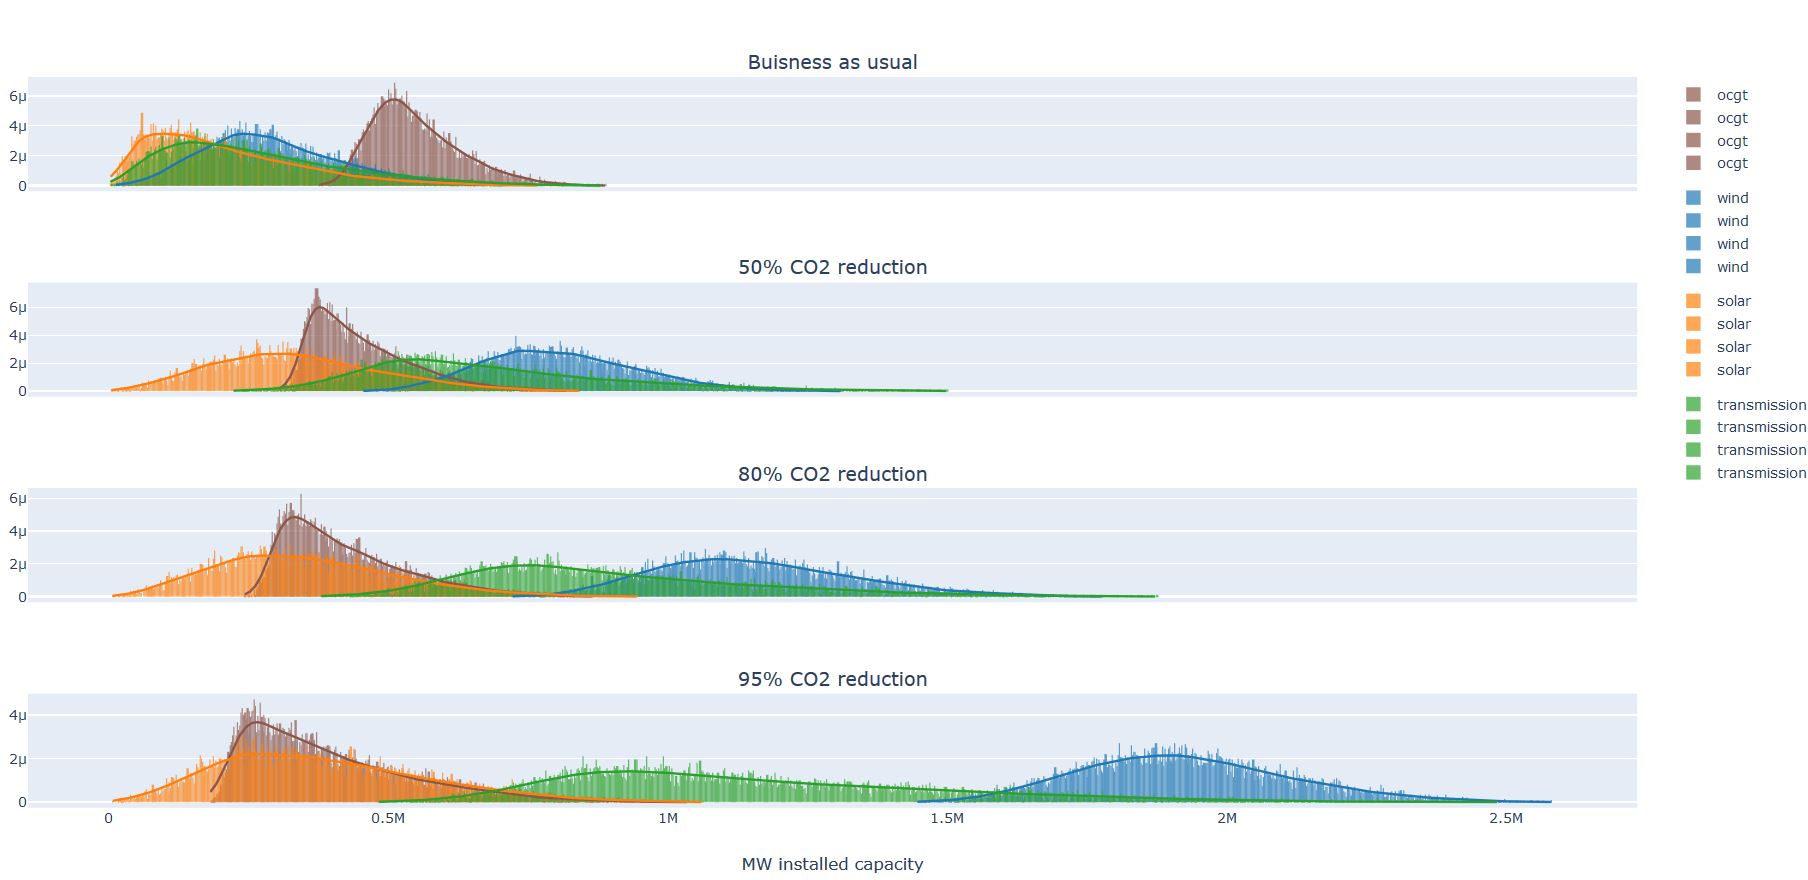
\includegraphics[width=1.2\textwidth,trim={0 1.5cm 0 0cm},clip]{./Images/4D_study_histogram}
	\caption{The figure shows the distribution of technology capacities for four MGA studies, where a MGA slack of 10\% have been used.}
	\label{fig:4d_hist}
\end{figure}


The distribution of capacities found in the four MGA studies is presented on figure \ref{fig:4d_hist}. As it was seen with the optimal solutions, the figure clearly shows how decreasing $\text{CO}_2$ emissions leads to an increase in wind and transmission capacity and a reduction in OCGT capacity. The results presented on figure \ref{fig:4d_hist}, furthermore provides information about the distribution of capacities. When analyzing the capacity distributions presented on \ref{fig:4d_hist} it is important to consider that there hasn't been accounted for multiplicity, meaning that the true distributions would be narrower, as discussed in section \ref{sec:Multiplicity}.

It is particularly interesting to see how the OCGT capacity distribution has a sharp lower bound, indicating that a rather fixed minimum amount of OCGT capacity is needed in all scenarios. The minimum OCGT capacity needed will be given by the remaining energy demand in the hour with the combined lowest availability of wind and solar power. In order to remove the need for backup generators such as gas turbines, would require unrealistically large capacities of wind and solar power. 

Figure \ref{fig:4d_hist} also shows how the distribution of capacities become wider as $\text{CO}_2$ emission is decreased. This essentially means that a larger configuration flexibility is available as $\text{CO}_2$ emissions is reduced. It could, however also be a result of how the MGA slack is defined. The MGA slack is defined as a percentage of the optimal solution scenario cost. As the cost of the optimal solutions varies a lot from the scenario with no $\text{CO}_2$ constraint to the scenario with tight $\text{CO}_2$ constraint, the allowable extra cost of scenarios also varies a lot, if measured in shear size and not as a percentage of the optimal solution objective value.

The distributions of solar power capacity in all four scenarios presented on figure \ref{fig:4d_hist}, all reach a value of 0 GW, meaning that solar power can be omitted if desired. In the scenarios with larger $\text{CO}_2$ reduction, this would however be a very extreme scenario, leading to a very specific design of the energy network. It is however not possible to configure a solution in a way that omits wind power in any of the four scenarios. 

\begin{figure}[h]\center
	\includegraphics[width=1\textwidth,trim={0 0cm 0 0cm},clip]{./Images/corelation_4D}
	\caption{This figure presents all variable correlations of the four MGA studies performed with 10\% MGA slack. Distributions of the four individual technologies are plotted on the diagonal, scatter plots of the data are shown in the lower left half and correlation values are presented in the upper right half of the plot matrix.}
	\label{fig:corelation}
\end{figure}

On figure \ref{fig:corelation} correlations of the four variables of the simplified decision space is shown. Data from all MGA studies performed have been used to generate this figure. 
The figure shows a strong correlation between wind power and transmission with a correlation of 0.50. This corresponds well with the results presented on figure \ref{fig:Optimal_Solutions}, where reinforcements on to the transmission grid is made as more wind is introduced to the model. Similar correlations between large shares of wind power and transmission capacity has been found in an article investigating this subject \cite{PURVINS20111461}. On the other hand, when analyzing the correlation between transmission and solar power a small negative correlation of -0.07 is found. This could suggest that the solar capacities installed, only produce enough energy to supply the country wherein they are installed, and therefore a need to transmit electricity generated by solar power doesn't exist. The correlation between energy production from solar PV in different countries has been studied in \cite{SolarPV_transmission}, where a strong correlation between production periods was found. As sunrise and sunset are similar in all European countries, the production of energy from solar PV happens simultaneously across entire Europe. Therefore an increase in transmission capacity would not allow more solar PV capacity to be installed. These results from \cite{SolarPV_transmission}, corresponds very well with whats seen in this project. 
A very strong negative correlation between OCGT and transmission is also presented on figure \ref{fig:corelation} with a correlation of -0.33. The capacity factor of OCGT does not depend on geographically determined factors and therefore OCGT capacity is installed where it is needed, leading to a negative correlation with transmission capacity.  
Another strong negative correlation is between wind power and OCGT with a value of -0.33. These two technologies appear to compete somewhat equally as energy sources.  


Analyzing the correlations of a single MGA study, namely the one with a $\text{CO}_2$ constraint of 95\% presented on figure \ref{fig:corelation_2}, it is a completely different story. Here the most significant correlation is between wind and solar power, that has a negative correlation of -0.72. This indicates that when a specific $\text{CO}_2$ reduction is desired, wind and solar power competes evenly as energy generating technologies. 
It is interesting to see how wind power and transmission has a small negative correlation when the correlations are calculated for just a single MGA study, compared to the large positive correlation, when data from all scenarios was considered. 


\begin{figure}[h]\center
	\includegraphics[width=1.\textwidth,trim={0 0cm 0 0cm},clip]{./Images/corelation_4D_95}
	\caption{The figure shows all variable correlations of the MGA study with a $\text{CO}_2$ emission reduction of 95\%. Distributions of the four individual technologies are plotted on the diagonal, scatter plots of the data are shown in the lower left half and correlation values are presented in the upper right half of the plot matrix.}
	\label{fig:corelation_2}
\end{figure}

In this project cost have been treated as one combined cost for the entire European energy network. This is however a very large simplification of the problem. In reality energy system cost is treated on national level, and therefore it is desired to distribute the energy system cost as evenly across all countries in the model. In this project the Gini coefficient is used as a measure for the equality of energy production versus consumption. This Gini coefficient can also be used as a measure of the equality in the distribution of system cost. 


\begin{figure}[h]\centering
	\begin{subfigure}{1\textwidth}
		\includegraphics[width=.9\textwidth,trim={0 0.8cm 0 2.5cm},clip]{./Images/corelation_gini_co2}
		\caption{}
		\label{fig:gini_co2}
	\end{subfigure}%
	\vspace{-.5cm}
	\begin{subfigure}{1\textwidth}
		\includegraphics[width=1\textwidth,trim={0 0.8cm 0 2.5cm},clip]{./Images/corelation_mix_co2}
		\caption{}
		\label{fig:mix_co2}
	\end{subfigure}%
	\label{fig:derivative_correlations}
	\caption{Figure (a) plots the Gini coefficient versus the reduction in $\text{CO}_2$ emissions. Figure (b) plots the wind/solar mix $\alpha$ versus the reduction in $\text{CO}_2$ emissions.}
\end{figure}

On figure \ref{fig:gini_co2} the Gini coefficient for all studies performed in this experiment is plotted against the $\text{CO}_2$ reduction. On the figure it is seen that there is a very strong positive correlation between $\text{CO}_2$ reduction and the Gini coefficient. This means that as requirements to reductions in $\text{CO}_2$ emissions increase, more energy needs to be produced in outside the countries where it is needed. A larger Gini coefficient also means that some countries will have to invest more money in modernizing the energy grid by installing larger capacities of renewable energy sources, and other countries will be depending on import of energy from countries with large capacities of renewable energy. As a country it is desired to be self sufficient with energy as energy is one of the most critical resources. The desire to reduce the Gini coefficient might therefore introduce a larger financial willingness. On figure \ref{fig:gini_co2}, it is seen that a 1\% slack on total system cost requires a Gini coefficient of at less 0.5 for a $\text{CO}_2$ reduction of 95\%, but increasing the slack to 10\% allows for a Gini coefficient as low as 0.3 for the same reduction in $\text{CO}_2$ emissions.  

In this study, the only variable renewable energy sources included are the two major variable renewable energy technologies, wind and solar power. From the correlation plot on figure \ref{fig:corelation}, as slight negative correlation with a value of -0.11 was seen. Such a small correlation value indicates that these two technologies interfere very little with each other, and that the share of wind and solar power remain somewhat constant. On figure \ref{fig:mix_co2}, the share of wind and solar power is plotted against $\text{CO}_2$ emissions. The share of wind and solar power $\alpha$ is calculated as the wind capacity relative to the total capacity of variable renewable energy. 

\begin{equation}
	\alpha =  \frac{\text{wind capacity}}{\text{wind capacity}+\text{solar capacity}}
\end{equation}

On figure \ref{fig:mix_co2} it is seen that the wind solar mix has an average around 0.8, complying very well with the results from \cite{rasmussen2011a}, where the mix of wind and solar power was studied. The penetration of wind power increases as $\text{CO}_2$ emissions decrease, which complies well with the results seen in the optimal solutions on figure \ref{fig:Optimal_Solutions_produc}, where implementation of solar PV capacity stagnates at $\text{CO}_2$ reduction levels higher than 50\%. Figure \ref{fig:mix_co2}, further shows that with a slack of 10\% on total system cost a wide span is available in the wind solar mix. At 95\% $\text{CO}_2$ reduction, it is possible to have a scenario that is 100\% wind dominated or a scenario where 50/50 mix between wind and solar is used. 

Having analyzed the results from this experiment, it can be concluded that the developed MGA algorithm is capable of providing useful insights regarding the techno-economic model investigated. Information that would not have been made available with other methods was extracted allowing for great insights regarding the possibilities available within the near optimal feasible space. 

\section{MGA study using seven decision variables}\label{sec:7D}
In the previous experiment, variables was grouped by technology type. It is however possible to group the variables in any way desired. Therefore a study investigating the interplay between energy production in North and South Europe has been performed, grouping the variables not only by technology type, but also by spatial location. A total of 7 grouped variables is formed, including OCGT, wind and solar power from both north and south Europa, and the total amount of transmission capacity. The grouped variables then becomes: 

\begin{equation*}
 \mathbf{x} = 
 \begin{Bmatrix}
 	x_1:& \text{North OCGT} \\
 	x_2:& \text{North wind} \\
 	x_3:& \text{North solar} \\
 	x_4:& \text{South OCGT} \\
 	x_5:& \text{South wind} \\
 	x_6:& \text{South solar} \\
 	x_7:& \text{Transmission} 
 \end{Bmatrix}
\end{equation*}

\begin{figure}[h]\centering
	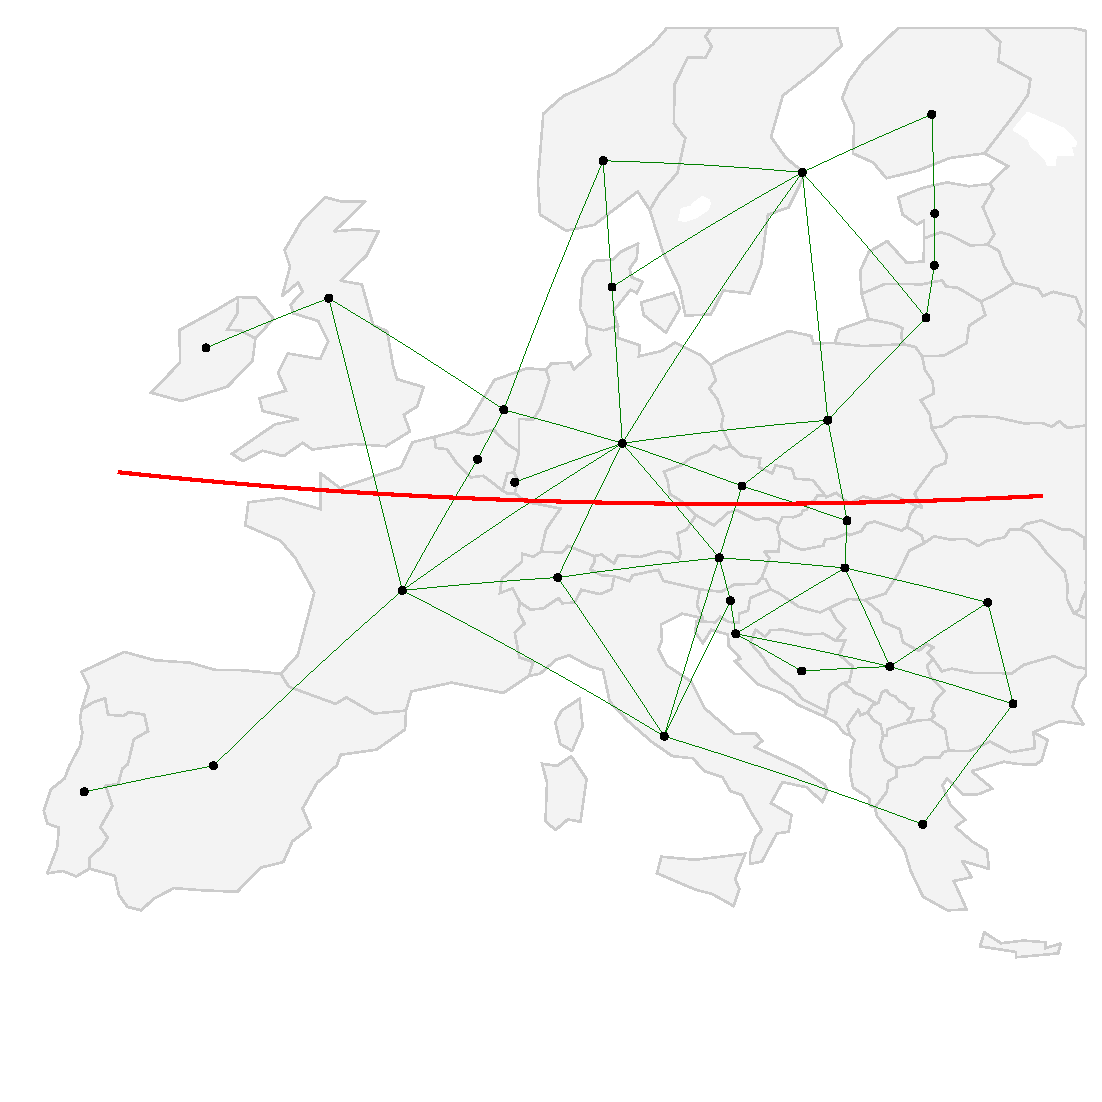
\includegraphics[width=.7\textwidth,trim={0 3cm 0 0cm},clip]{./Images/7D_study_topology}
	\caption{The figure shows the topology of the techno-economic model used in the study. The red line indicates the parting line between north and south Europe. }
	\label{fig:7d_topology}
\end{figure}

A parting line between north and south Europe was drawn at latitude 49.2421, which is equivalent to the median of the latitude position of all country centroids included in the model. All countries with a centroid north of latitude 49.2421 is considered as north Europe, and all other countries are considered as south Europe. A total of 15 countries are included in each category. The parting line is presented on figure \ref{fig:7d_topology}. 

\begin{figure}[p]\centerfloat
	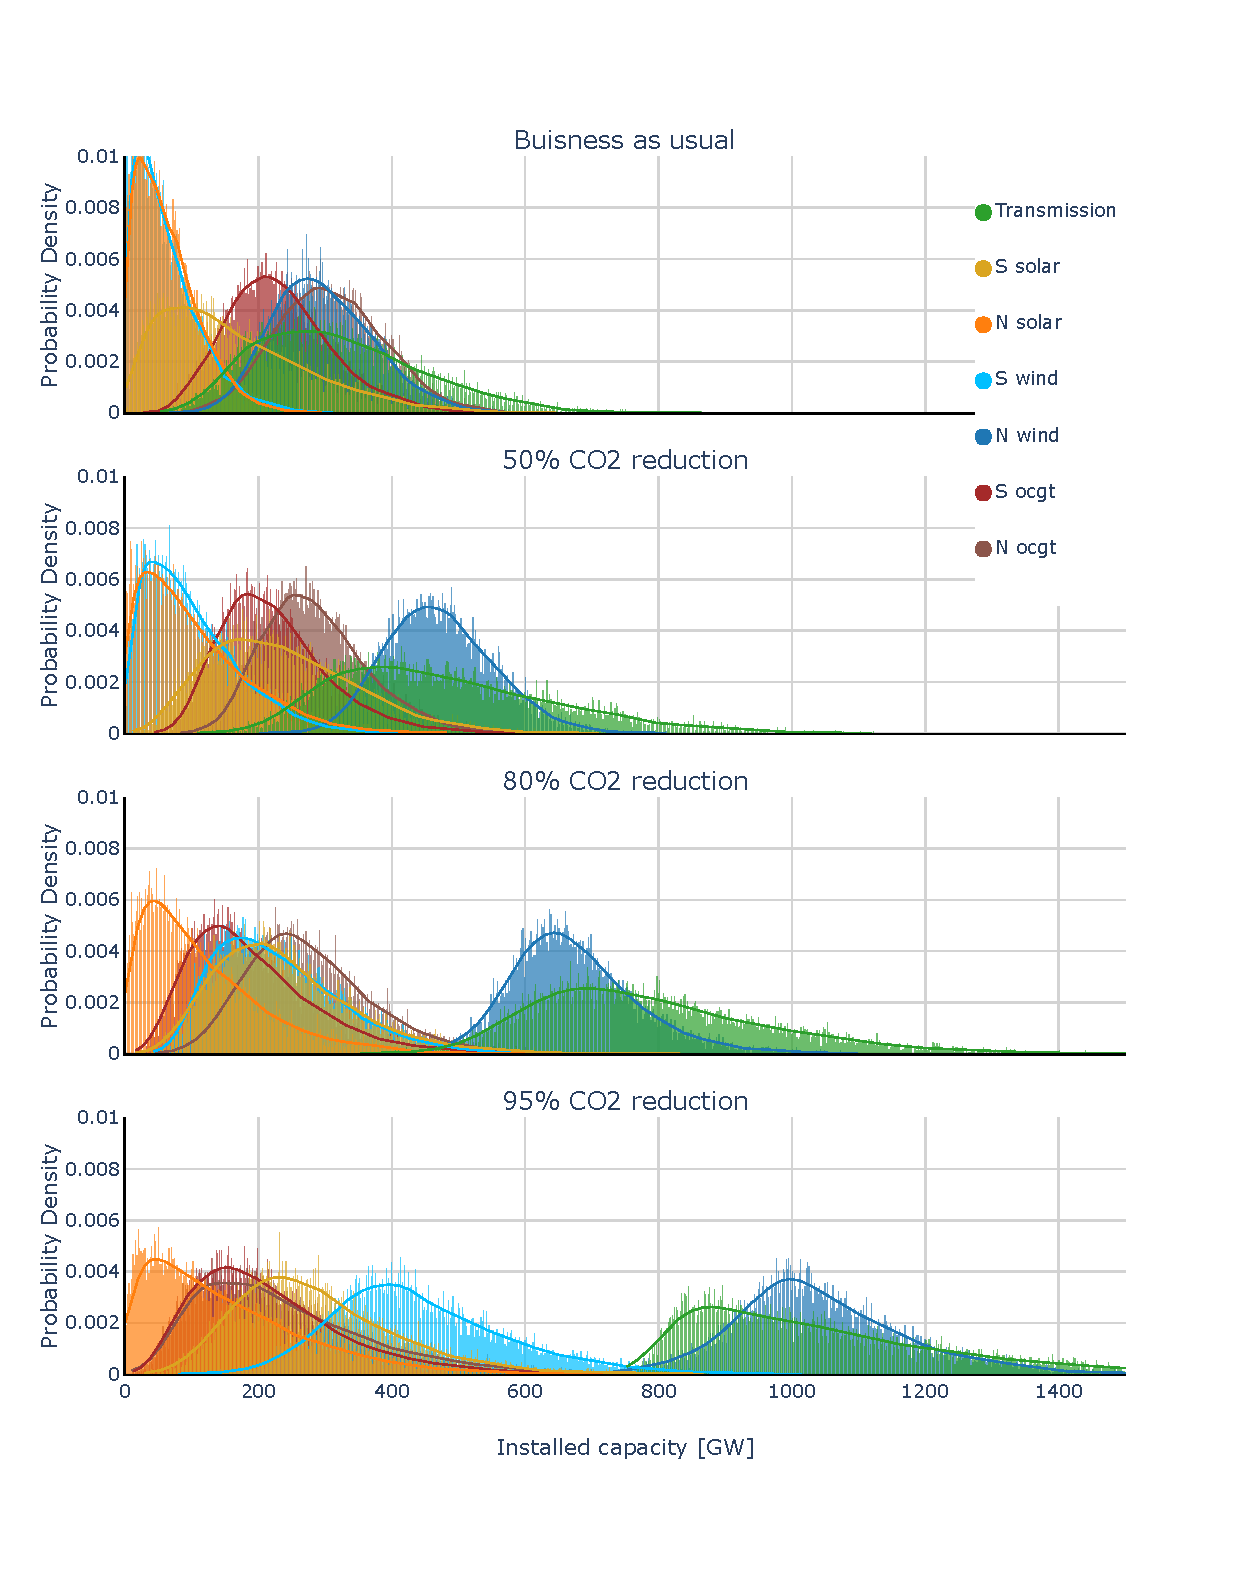
\includegraphics[width=1.3\textwidth,trim={0 1.7cm 0 0cm},clip]{./Images/7D_study_histogram}
	\caption{The figure shows the distribution of technology capacities for four MGA studies, where a MGA slack of 10\% have been used, and seven variables has been included in the MGA study. }
	\label{fig:7d_hist}
\end{figure}

Using the novel MGA method presented in this project, the capacities of all near optimal solutions was found, using a MGA slack of 10\% on four scenarios with respectively 0, 50, 80 and 95\% reduction in $\text{CO}_2$ emissions. 

On figure \ref{fig:7d_hist}, a histogram presenting all seven grouped variables for all four scenarios is shown. Much like the study performed using only four grouped variables seen on figure \ref{fig:4d_hist}, the wind and solar capacities increase as $\text{CO}_2$ emissions are reduced.  
Analyzing the data presented on figure \ref{fig:7d_hist}, it is clearly seen that wind power in northern Europe is preferred over any other energy generating technologies, as $\text{CO}_2$ emissions are lowered. Comparing solar power in north and south Europe, it is seen that south Europe in all scenarios have a larger amount of installed capacity. Scenarios where large shares of solar power is installed in north Europe is however also feasible, and in a scenario where $\text{CO}_2$ emissions are reduced by 95\%, a scenario with 600GW of installed solar capacity in north Europe wold be feasible. 

Analyzing the distributions of wind and solar power on figure \ref{fig:7d_hist}, it is seen that there is an overlap between respectively wind in north and south Europe, and solar power in north and south Europe. This shows, that a scenario with more solar capacity in northern Europe compared to south Europe is feasible with a 10\% slack on cost, or a scenario with more wind in southern Europe than northern Europe. 

Analyzing the correlations presented on figure \ref{fig:7d_corr}, results show a significant correlation between wind and transmission. Especially wind in north Europe has a strong correlation with transmission, with a correlations above 0.4. Wind power in south Europe correlates positive with transmission too, only with a correlation factor of 0.12. 
The results presented on figure \ref{fig:7d_corr}, further shows strong negative correlations between OCGT in north and south Europe, indicating that OCGT in north Europe competes very directly with OCGT power in south Europe. A similar tendency is seen between solar power in north and south Europe. Interestingly, no correlation is seen between wind in north and south Europe, indicating that the installed capacity of wind in either end of Europe, has no effect on each other. 

\begin{figure}[h]\centerfloat
	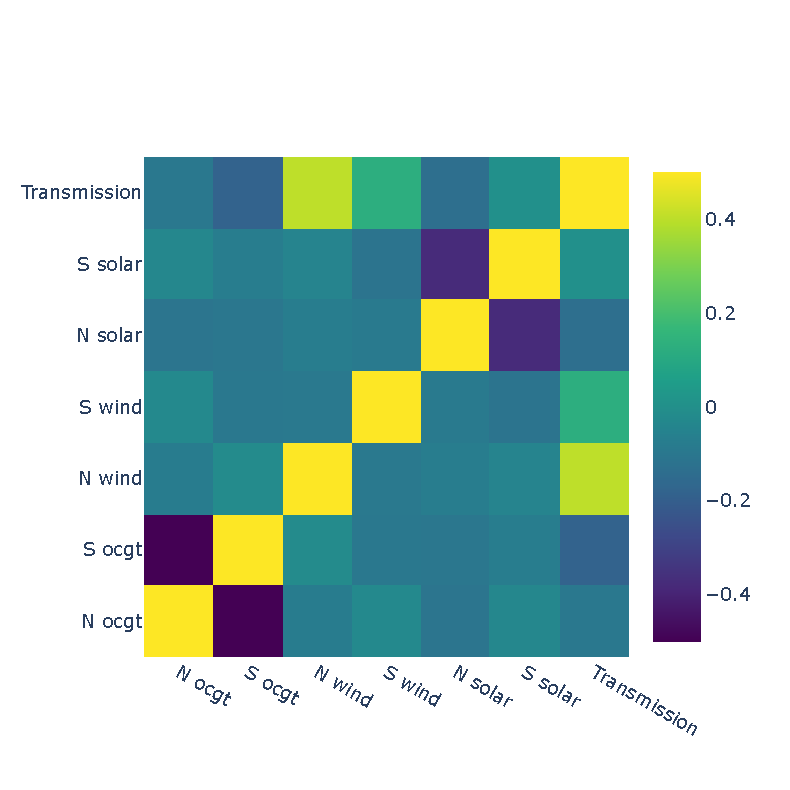
\includegraphics[width=0.8\textwidth,trim={0 .5cm 0 2cm},clip]{./Images/7D_study_corr}
	\caption{The figure shows a heatmap representing the correlation matrix of the variables in the four MGA studies performed with seven variables included in the study.}
	\label{fig:7d_corr}
\end{figure}

Each of the four studies performed in this experiment required 48 hours of computing time on the PRIME computing cluster \cite{Prime} using a single 32 core computing node. Including more variables in the decision space considered by the MGA algorithm is possible but the practical maximum is estimated to be roughly 10 decision variables.  

\section{Comparison of MGA algorithms}\label{sec:MGA_comparisons}
The goal of this experiment is to highlight the benefits and weakness of existing MGA methods compared to the novel MGA approach presented in this project. The following four different MGA techniques will be explored: The HSJ approach presented in \cite{DeCarolis_MGA}, an approach where groups of variables are maximized and minimized presented in \cite{Fabian_MGA} together with an approach where all decision variables are maximized and minimized and the novel approach presented in this project. 

\begin{figure}[h]\centering
	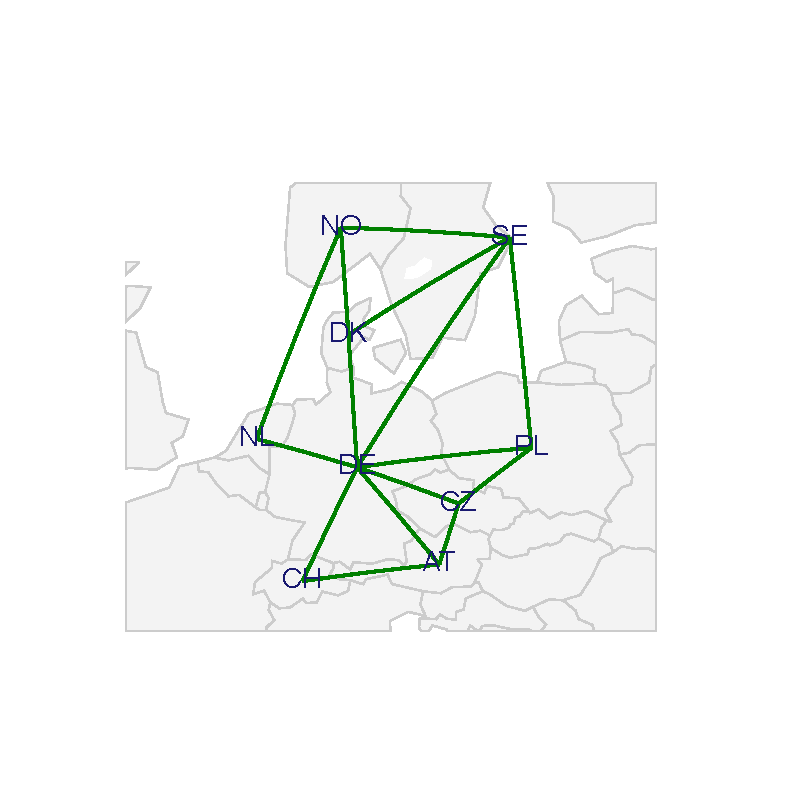
\includegraphics[width=.7\textwidth,trim={0 2.8cm 0 3cm},clip]{./Images/comparison_topology}
	\caption{The figure shows the topology of the simplified network used in study comparing performance of MGA algorithms. }
	\label{fig:comparison_topology}
\end{figure}


When comparing MGA approaches in this section, it is very important to keep in mind what to goal of performing an MGA analysis is, and what measure characterized a good MGA technique. The overall objective is to explorer the possibilities for alternative solutions to the optimization problem within a certain range of economical slack. Solutions to an techno-economic problem as the one considered in this project can however be different in a wide range of manners, as the decision space is high dimensional. This makes it hard to determine the coverage of the decision space for a given MGA method, as the extend of the decision space is unknown. Instead, the results found with the different MGA methods, will be analyzed, compared and discussed in an attempt to determine strengths, and weaknesses for the MGA methods. 

In order to generate comparable results, all four MGA methods are implemented on the same simplified network. As the focus of this experiment is to compare methods, and not to analyze an techno-economic model, a simplified model is used to reduce computation time needed, and complexity of the results. The techno-economic model used in this experiment includes only nine of the thirty countries from the full model as shown on figure \ref{fig:comparison_topology}. Furthermore, only a single 24 hour period is simulated. The result is a model with 27 variables (9 countries with 3 technologies each), when hourly dispatch is not considered as a decision variable. Furthermore, a $\text{CO}_2$ constraint is employed forcing the model to reduce $\text{CO}_2$ emissions with 80\% compared to an unrestricted scenario. 

\begin{figure}[h]\centering
	\begin{subfigure}{.5\textwidth}
		\includegraphics[width=1.\textwidth]{./Images/Comparison_1}
		\caption{}
		\label{fig:comparison_1}
	\end{subfigure}%
	%\vspace{10pt}
	\begin{subfigure}{.5\textwidth}
		\includegraphics[width=1.\textwidth]{./Images/Comparison_4}
		\caption{}
		\label{fig:comparison_2}
	\end{subfigure}%
	\vspace{1pt}
	\begin{subfigure}{.5\textwidth}
		\includegraphics[width=1.\textwidth]{./Images/Comparison_2}
		\caption{}
		\label{fig:comparison_3}
	\end{subfigure}%
	%\vspace{10pt}
	\begin{subfigure}{.5\textwidth}
		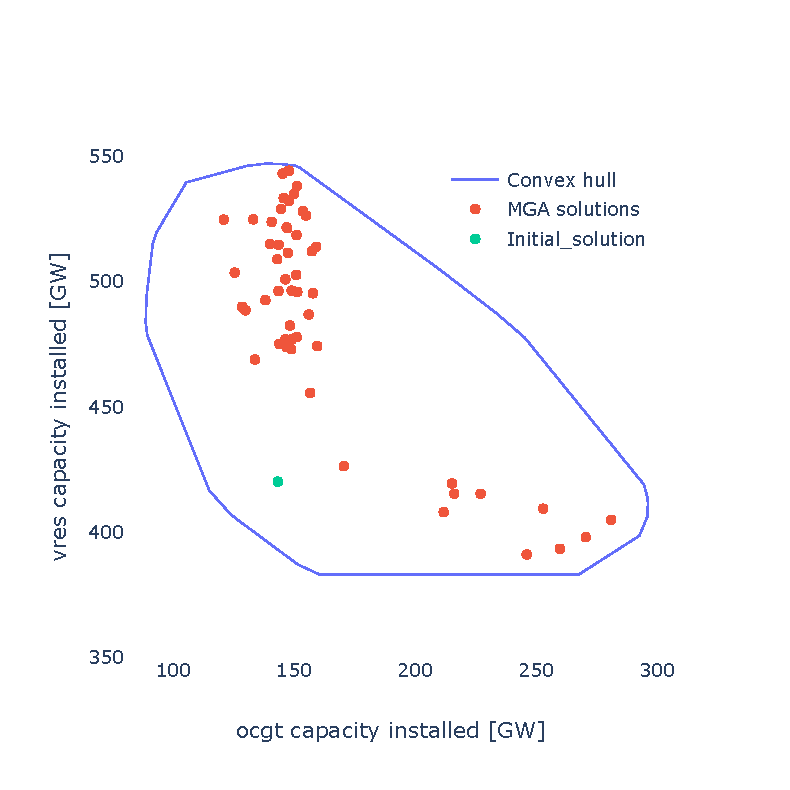
\includegraphics[width=1.\textwidth]{./Images/comparison_3}
		\caption{}
		\label{fig:comparison_4}
	\end{subfigure}
	\caption{On the figure the found MGA solutions within the reduced decision space of four MGA algorithms is presented. Figure (a) presents the results from the novel MGA method. Figure (b) shows the results from the maximization and minimization of grouped variables approach, as presented in \cite{Fabian_MGA}. Figure (c) presents results from the HSJ MGA method from \cite{DeCarolis_MGA}, and figure (d) shows the results from the maximization and minimization of all decision variables as presented in \cite{Fabian_MGA}.}
	\label{fig:comparison_results}
\end{figure}

Using the approach presented in section \ref{sec:dim_reduction} to reduce the dimensionality, a new two-dimensional decision space is formed, by grouping the variables in a group representing all installed gas turbine capacity and the other group representing all variable renewable energy source capacity (wind and solar power). This allows for easy visualization and understanding of the results. 

Initially the novel MGA approach presented in this project, was deployed to find the convex hull containing all solutions in the two-dimensional decision space. As this method converges towards the full solution, the result can be considered as the full solution to the two-dimensional problem. The found convex hull is presented in figure \ref{fig:comparison_1}. The shaded area of the convex hull indicates that the novel MGA approach extracts information about the entire hull volume in regard to all other MGA approaches that terminates when a set of different solution is found. Despite using a simplified techno-economic model and reducing dimensionality to just two dimensions, the shape of the convex hull is still rather complex. 

 



On figure \ref{fig:comparison_2}, the results of the method from \cite{Fabian_MGA} where the grouped decision variables are maximized and minimized, is presented. This method effectively performs the same initial MGA iteration as the novel MGA approach, and therefore it finds solutions also found be the novel MGA approach. In the work presented in \cite{Fabian_MGA}, these maximized and minimized solutions are used to create upper and lower bounds on the summarized capacities. Four individual solutions found using this technique is presented on figure \ref{fig:MGA_sum_results}. 


\begin{figure}[h]\centering
	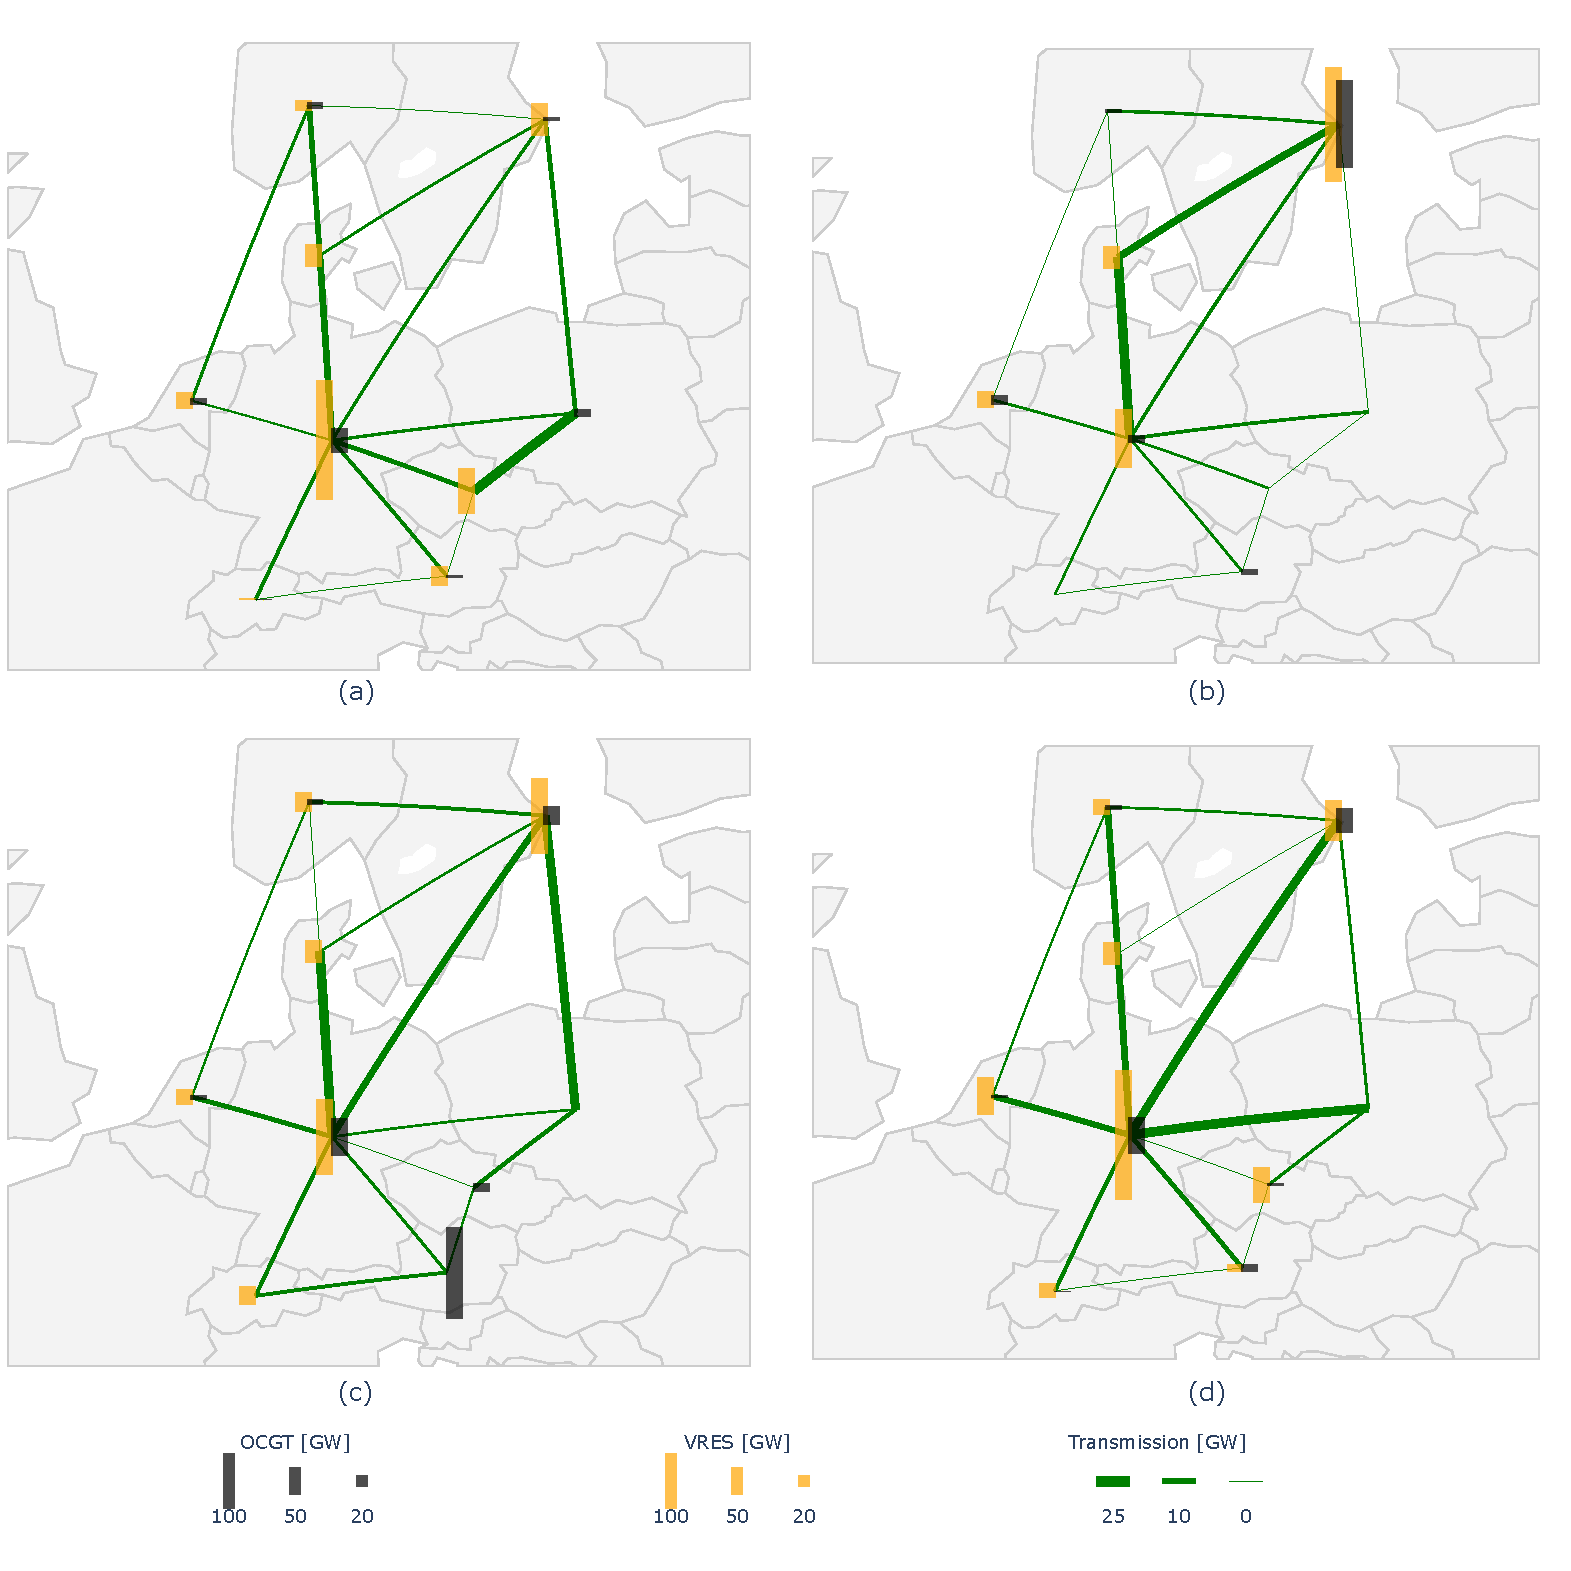
\includegraphics[width=1.\textwidth,trim={0 0cm 0 0cm},clip]{./Images/MGA_sum}
	\caption{On the figure a presentation of capacity distributions from four solutions using the novel MGA results is presented. The four studies have used the following objective functions: (a) Minimize OCGT, (b) Minimize VRES, (c) Maximize OCGT, (d) Maximize VRES}
	\label{fig:MGA_sum_results}
\end{figure}


Analyzing the result of the HSJ MGA method on figure \ref{fig:comparison_3}, it is clear that it does not search towards the edge of the convex hull as the first two methods. The reason hereof is that the HSJ method doesn't consider the grouped variables. Instead, it seeks to create maximally different solutions by implementing technologies not included in the previous solution. Here similar technologies from different countries are treated as two individual technologies. Analyzing the individual HSJ solutions presented on figure \ref{fig:HSJ_results} they are very different. Although all the solutions implement similar capacities of VRES and OCGT when summarized, the placement of the capacity implemented varies a lot from solution to solution. Looking at the two HSJ solutions from figure \ref{fig:HSJ_results}b and \ref{fig:HSJ_results}c, where solution (b) implements all VRES in Denmark and Germany, and solution (c) implements no VRES in Germany, but spreads it to the surrounding countries, it is easy to see that the solutions are topologically different but when analyzing the summarized capacities they are very similar. 

\begin{figure}[h]\centering
	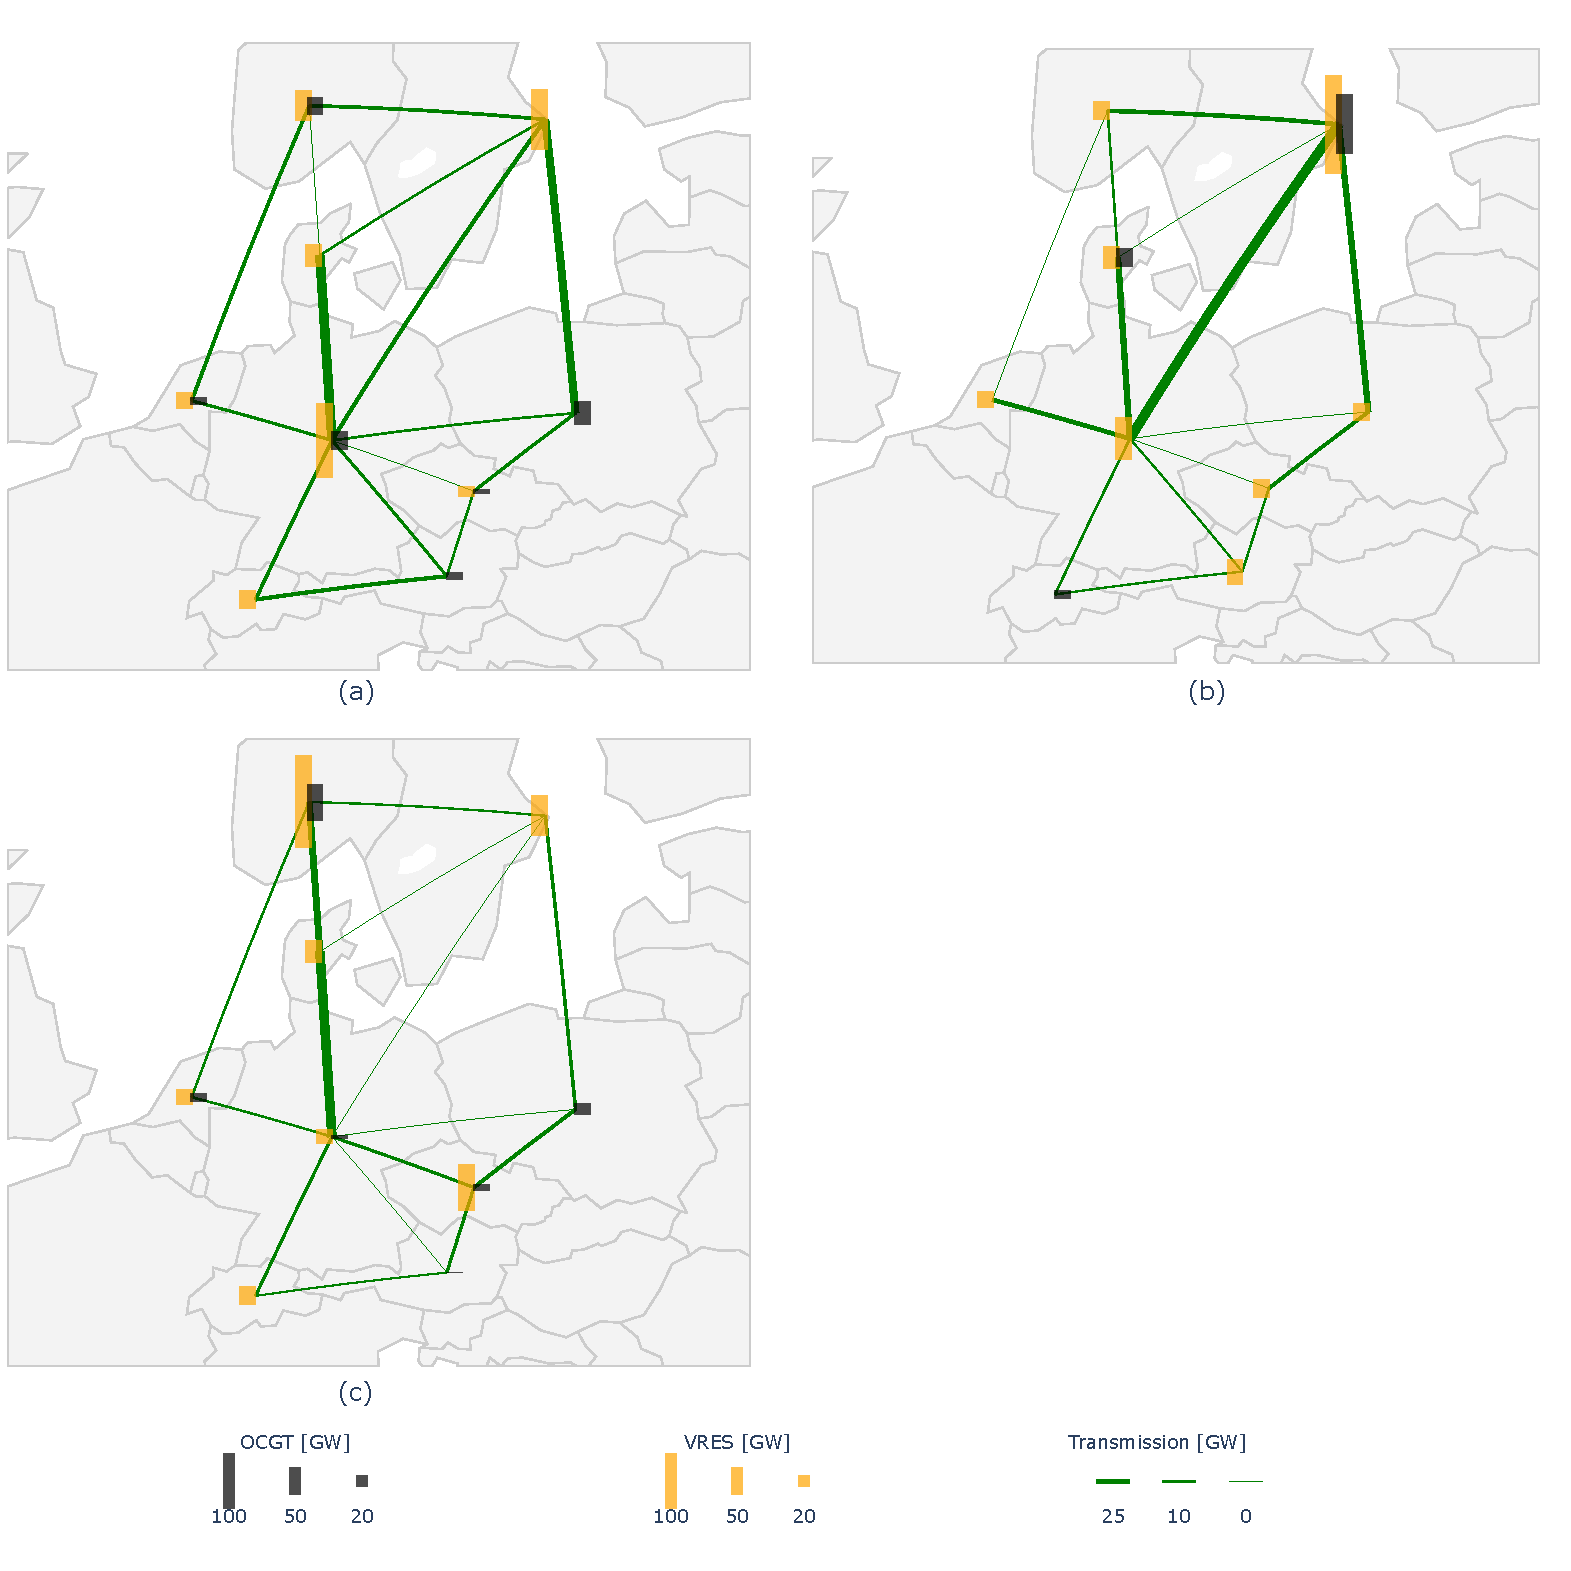
\includegraphics[width=1.\textwidth,trim={0 0cm 0 0cm},clip]{./Images/HSJ}
	\caption{On the figure a presentation of capacity distributions from three solutions using the novel HSJ MGA method is presented. Figure (a) shows the optimal solution, and figure (b) and (c) are HSJ solutions. }
	\label{fig:HSJ_results}
\end{figure}

The overall conclusion from this study must be that the novel MGA approach developed in this project shows to be very effective in its ability to determine the shape of the near optimal feasible space. Although it performs more optimizations than the other MGA methods, it uses these optimization runs wisely to investigate complex regions of the decision space. 



%\clearpage

\chapter{Discussion}

Why high dim are so hard to deal with.
%\clearpage

\chapter{Conclusion}


%\clearpage

%

\chapter*{Notes on references}

\subsubsection*{Impact of CO2 prices on the design of a highly decarbonized coupled
electricity and heating system in Europe\cite{PypsaModel}}
An investigation on the CO2 price levels needed to reduce CO2 emissions. In the article a PyPSA model of Europe is presented. The model could be used in this project. 

\subsubsection*{MODELING TO GENERATE ALTERNATIVES: THE HSJ
APPROACH AND AN ILLUSTRATION USING A
PROBLEM IN LAND USE PLANNING \cite{Brill_MGA_1982}}

This is the original article, \cite{Brill_MGA_1982}, explaining the thoughts behind MGA. In this article the HSJ (Hop Skip Jump) approach is implemented. This article seams to be the mother of all other MGA articles. 

\subsubsection*{MGA: a decision support system for complex, incompletely defined problems\cite{Brill_MGA_1990}}
Elaborating on the MGA approach presented in \cite{Brill_MGA_1982}, and evaluating the performance of MGA as a whole. 

\subsubsection*{Using modeling to generate alternatives (MGA) to expand our thinking on
energy futures\cite{DeCarolis_MGA}}

\cite{DeCarolis_MGA} is one of the first implementations of MGA on energy planning. Uses the HSJ method from \cite{Brill_MGA_1982}.

\subsubsection*{Modeling to generate alternatives: A technique to explore uncertainty
in energy-environment-economy models \cite{MGA}}

In this article MGA is used to explore near optimal solutions in energy network optimization, much like \cite{DeCarolis_MGA}. However a slightly more advanced MGA objective function is used. The objective function to be maximized is the Manhattan distance between the current and all preveiously generated MGA solutions. 

\subsubsection*{Ensuring diversity of national energy scenarios: Bottom-up energy
system model with Modeling to Generate Alternatives \cite{BERNTSEN2017886}}
A different approach towards implementing MGA on energy system planning. Here they use the  EXPANSE software/model to implement MGA on. They use a sort of random search MGA approach.

\subsubsection*{Simulation-Optimization techniques formodelling to generate alternatives in waste management planning \cite{Yavuz2011}}
This article describes the MGA method used in \cite{BERNTSEN2017886}. Here a random population is created and is sorted through a number of itterations. 

\subsubsection*{GENETIC ALGORITHM APPROACHES FOR ADDRESSING UNMODELED OBJECTIVES IN OPTIMIZATION PROBLEMS \cite{Genetic_Algorithms_for_MGA}}
This article describes the basic theory of MGA very well, and introduces two new genetic algorithms, that could be used for MGA. The Algorithms are based on genetic nieching/sharing algorithms. 

\subsubsection*{A Co-evolutionary, Nature-Inspired Algorithm for the Concurrent Generation of Alternatives \cite{FireFly_MGA_Article}}

The article \cite{FireFly_MGA_Article} describes an implementation of the genetic firefly algorithm used to perform MGA. 

\subsubsection*{Swarm Intelligence and Bio-Inspired Computation : Theory and Applications - Chapter 14 \cite{Bio_computation_book}}

The book \cite{Bio_computation_book} Chapter 14 describes the firefly algorithm in depth an has multiple examples of the firefly algorithm implemented. The book cites \cite{FireFly_MGA_Article} . 

\subsubsection*{The benefits of cooperation in a highly renewable European electricity network \cite{PypsaModel}}
Article describing simulations using the PyPSA-EUR-30 model. There is a great explanation of the math behind PyPSA 

\subsubsection*{Transmission needs across a fully renewable European power system}
\cite{RODRIGUEZ2014467}
Article exploring the effect of transmission across the EURO-30 model. 

\subsubsection*{Validation of Danish wind time series from a new global renewable energy atlas for energy system analysis}
\cite{ANDRESEN20151074} REAtlas software

\subsubsection*{The NCEP Climate Forecast System Version 2}
\cite{ClimateForecastSystem} Weather data

\subsubsection*{The role of spatial scale in joint optimisations of generation and transmission for European highly renewable scenarios\cite{spatialInfluence} }
An article exploring the influence of spatial simplification on energy models. An exapmle using k-means to perform spatial simplification is shown.  

\subsubsection*{Modelling to generate alternatives with an energy system optimization model \cite{DECAROLIS2016}}
Another article by DeCariolis exploring the HSJ MGA methodology on energy system optimization 

\subsubsection*{The optimum is not enough: A near-optimal solution paradigm for energy systems synthesis \cite{Optimum_not_enough}}
A different approach for exploring the near optimal feasable space, using a technique that is not quite MGA but very similar. The approach generates a finite set of alternative solutions. 


\subsubsection*{Current and prospective costs of electricity generation until 2050}
\cite{Schroder2013Current} includes cost data for all energy technologies relevant for this study

\subsubsection*{Optimal Combination of Storage and Balancing in a 100\% Renewable European Power System}
\cite{rasmussen2011a}
Article where the optimal mix between wind and solar energy is explored. 



%\clearpage


\begingroup
%	\raggedright
\bibliography{references}	
%\bibliography{sample}				
\endgroup

%\printbibliography[heading=head]




\appendix
\clearpage
\startlist{toc}
\printlist{toc}{}{\part{Appendix}}
%\addtocontents{toc}{part}{Appendiks}
%Nedenfor indsættes appendiks
\setcounter{chapter}{0}
\renewcommand{\thechapter}{\Alph{chapter}}


\chapter{Code}


All written code for this project can be found on Github at \url{https://github.com/TimToernes/MGA-PyPSA}. 


\subsection{Pseudo code}

\begin{enumerate}[label={}]
\item Solve network subject to regular constraints and with original objective function
\item Add MGA constraint !Equation number
\item while $\epsilon>tol$
\begin{itemize}[label={}]
\item If first loop
\begin{itemize}[label={}]
\item directions = max and min all variables
\end{itemize}
\item Else
\begin{itemize}[label={}]
\item directions = normals to hull faces
\end{itemize}
\item for direction in directions
\begin{itemize}[label={}]
\item objective function = direction[i] * variable[i]
\item point on convex hull += solve problem subject to objective function
\end{itemize}
\item hull = ConvexHull ( points on convex hull)
\item $epsilon$ = new hull volume - old hull volume / hull volume
\end{itemize}
\item Evenly distribute points in hull 
\item Plot histogram using evenly distributed points. 
\end{enumerate}




\chapter{Plots for section \ref{sec:4D} }

\begin{figure}[p]\center
	\includegraphics[width=1.2\textwidth,trim={0 0cm 0 0cm},clip]{./Images/corelation_4D_00}
	\caption{Variable correlations of the MGA study with a CO2 emission reduction of 0\%. Distributions of the four individual technologies are plotted on the diagonal.}

\end{figure}

\begin{figure}[p]\center
	\includegraphics[width=1.2\textwidth,trim={0 0cm 0 0cm},clip]{./Images/corelation_4D_50}
	\caption{Variable correlations of the MGA study with a CO2 emission reduction of 50\%. Distributions of the four individual technologies are plotted on the diagonal.}

\end{figure}

\begin{figure}[p]\center
	\includegraphics[width=1.2\textwidth,trim={0 0cm 0 0cm},clip]{./Images/corelation_4D_80}
	\caption{Variable correlations of the MGA study with a CO2 emission reduction of 80\%. Distributions of the four individual technologies are plotted on the diagonal.}

\end{figure}

\begin{figure}[p]\center
	\includegraphics[width=1.2\textwidth,trim={0 0cm 0 0cm},clip]{./Images/corelation_4D}
	\caption{Variable correlations of the MGA study with a CO2 emission reduction of 95\%. Distributions of the four individual technologies are plotted on the diagonal.}

\end{figure}




\begin{figure}[p]\raggedleft
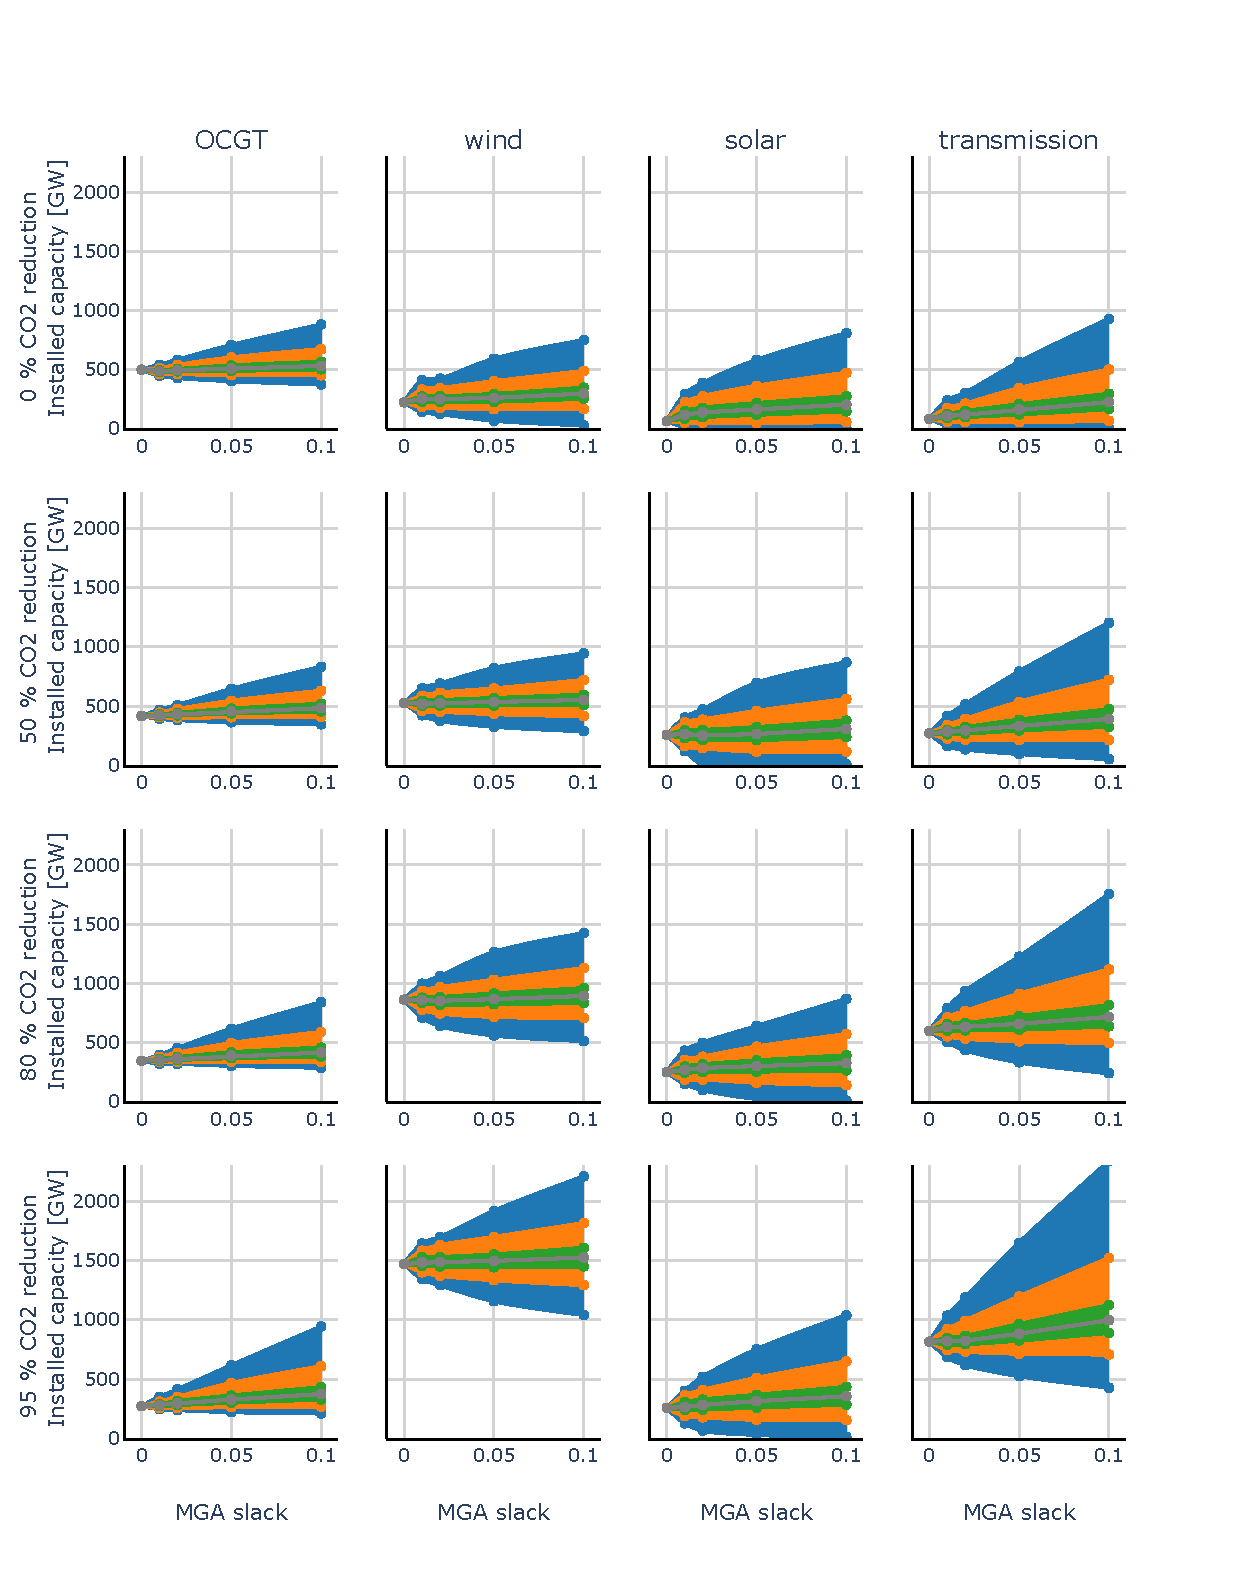
\includegraphics[width=.9\paperwidth,trim={0 0cm 0 0cm},clip]{./Images/Capacaty_vs_cost}
\label{fig:cap_vs_cost}
\caption{text}
\end{figure}
	%OK


\end{document}














%%%%%%%%%%%%%%%%%%%%%%%%%%%%%%%%%%%%%%%%%%%%%%%
%minifigures
\begin{figure}[H]
  \centering
  \begin{minipage}[b]{0.48\textwidth}
    \includegraphics[width=\textwidth]{metalmapel_Cu-K.jpg}
    \caption{Marked Copper in the sample}
  \end{minipage}
  \hfill
  \begin{minipage}[b]{0.48\textwidth}
    \includegraphics[width=\textwidth]{metalcarto.jpg}
    \caption{Marked Copper, Silver and Iron in the sample}
  \end{minipage}
\end{figure}